\documentclass[twoside]{book}

% Packages required by doxygen
\usepackage{fixltx2e}
\usepackage{calc}
\usepackage{doxygen}
\usepackage[export]{adjustbox} % also loads graphicx
\usepackage{graphicx}
\usepackage[utf8]{inputenc}
\usepackage{makeidx}
\usepackage{multicol}
\usepackage{multirow}
\PassOptionsToPackage{warn}{textcomp}
\usepackage{textcomp}
\usepackage[nointegrals]{wasysym}
\usepackage[table]{xcolor}

% Font selection
\usepackage[T1]{fontenc}
\usepackage[scaled=.90]{helvet}
\usepackage{courier}
\usepackage{amssymb}
\usepackage{sectsty}
\renewcommand{\familydefault}{\sfdefault}
\allsectionsfont{%
  \fontseries{bc}\selectfont%
  \color{darkgray}%
}
\renewcommand{\DoxyLabelFont}{%
  \fontseries{bc}\selectfont%
  \color{darkgray}%
}
\newcommand{\+}{\discretionary{\mbox{\scriptsize$\hookleftarrow$}}{}{}}

% Page & text layout
\usepackage{geometry}
\geometry{%
  a4paper,%
  top=2.5cm,%
  bottom=2.5cm,%
  left=2.5cm,%
  right=2.5cm%
}
\tolerance=750
\hfuzz=15pt
\hbadness=750
\setlength{\emergencystretch}{15pt}
\setlength{\parindent}{0cm}
\setlength{\parskip}{3ex plus 2ex minus 2ex}
\makeatletter
\renewcommand{\paragraph}{%
  \@startsection{paragraph}{4}{0ex}{-1.0ex}{1.0ex}{%
    \normalfont\normalsize\bfseries\SS@parafont%
  }%
}
\renewcommand{\subparagraph}{%
  \@startsection{subparagraph}{5}{0ex}{-1.0ex}{1.0ex}{%
    \normalfont\normalsize\bfseries\SS@subparafont%
  }%
}
\makeatother

% Headers & footers
\usepackage{fancyhdr}
\pagestyle{fancyplain}
\fancyhead[LE]{\fancyplain{}{\bfseries\thepage}}
\fancyhead[CE]{\fancyplain{}{}}
\fancyhead[RE]{\fancyplain{}{\bfseries\leftmark}}
\fancyhead[LO]{\fancyplain{}{\bfseries\rightmark}}
\fancyhead[CO]{\fancyplain{}{}}
\fancyhead[RO]{\fancyplain{}{\bfseries\thepage}}
\fancyfoot[LE]{\fancyplain{}{}}
\fancyfoot[CE]{\fancyplain{}{}}
\fancyfoot[RE]{\fancyplain{}{\bfseries\scriptsize Generated by Doxygen }}
\fancyfoot[LO]{\fancyplain{}{\bfseries\scriptsize Generated by Doxygen }}
\fancyfoot[CO]{\fancyplain{}{}}
\fancyfoot[RO]{\fancyplain{}{}}
\renewcommand{\footrulewidth}{0.4pt}
\renewcommand{\chaptermark}[1]{%
  \markboth{#1}{}%
}
\renewcommand{\sectionmark}[1]{%
  \markright{\thesection\ #1}%
}

% Indices & bibliography
\usepackage{natbib}
\usepackage[titles]{tocloft}
\setcounter{tocdepth}{3}
\setcounter{secnumdepth}{5}
\makeindex

% Hyperlinks (required, but should be loaded last)
\usepackage{ifpdf}
\ifpdf
  \usepackage[pdftex,pagebackref=true]{hyperref}
\else
  \usepackage[ps2pdf,pagebackref=true]{hyperref}
\fi
\hypersetup{%
  colorlinks=true,%
  linkcolor=blue,%
  citecolor=blue,%
  unicode%
}

% Custom commands
\newcommand{\clearemptydoublepage}{%
  \newpage{\pagestyle{empty}\cleardoublepage}%
}

\usepackage{caption}
\captionsetup{labelsep=space,justification=centering,font={bf},singlelinecheck=off,skip=4pt,position=top}

%===== C O N T E N T S =====

\begin{document}

% Titlepage & ToC
\hypersetup{pageanchor=false,
             bookmarksnumbered=true,
             pdfencoding=unicode
            }
\pagenumbering{alph}
\begin{titlepage}
\vspace*{7cm}
\begin{center}%
{\Large btosg }\\
\vspace*{1cm}
{\large Generated by Doxygen 1.8.13}\\
\end{center}
\end{titlepage}
\clearemptydoublepage
\pagenumbering{roman}
\tableofcontents
\clearemptydoublepage
\pagenumbering{arabic}
\hypersetup{pageanchor=true}

%--- Begin generated contents ---
\chapter{mainpage}
\label{md_mainpage}
\Hypertarget{md_mainpage}
A thin abstraction layer to integrate {\bfseries Bullet} and {\bfseries Open\+Scene\+Graph}.

\subsubsection*{Description}

{\bfseries btosg} is aimed to ease building simple visual simulation applications integrating {\bfseries Bullet} and {\bfseries Open\+Scene\+Graph}. {\bfseries btosg} stands on top of these two A\+P\+Is but does not try to hide them. Instead, in order to build a complete application, the programmer is able and usually needs to access directly the data structures from both {\bfseries Bullet} and {\bfseries Open\+Scene\+Graph}. So, the use of {\bfseries btosg} does not avoid the requirement to know and understand their A\+P\+Is.

The use of {\bfseries btosg} can help the programming task because it allows to create and position both the physical and graphics definitions of small objects in one step. It also keeps track of syncronizing the graphics definitions from the state of each physical object.

\subsubsection*{Dependences}

\paragraph*{Open\+Scene\+Graph\+:}


\begin{DoxyItemize}
\item \href{https://github.com/openscenegraph/OpenSceneGraph}{\tt https\+://github.\+com/openscenegraph/\+Open\+Scene\+Graph}
\item \href{http://www.openscenegraph.org/}{\tt http\+://www.\+openscenegraph.\+org/}
\end{DoxyItemize}

\paragraph*{Bullet\+:}


\begin{DoxyItemize}
\item \href{https://github.com/bulletphysics/bullet3}{\tt https\+://github.\+com/bulletphysics/bullet3}
\item \href{http://bulletphysics.org/}{\tt http\+://bulletphysics.\+org/}
\end{DoxyItemize}

Dependences can be installed on Fedora Linux using\+: \begin{DoxyVerb}dnf install bullet bullet-devel OpenSceneGraph OpenSceneGraph-devel
\end{DoxyVerb}


Dependences can be installed on Ubuntu using\+: \begin{DoxyVerb}apt install bullet openscenegraph-osg openscenegraph-osgViewer openscenegraph-osgSim openscenegraph-osgDB openscenegraph-osgGA openscenegraph-osgShadow
\end{DoxyVerb}


\subsubsection*{Build}

\begin{DoxyVerb}git clone https://github.com/miguelleitao/btosg.git
cd btosg
make
sudo make install
\end{DoxyVerb}


\subsubsection*{Usage}

Look at provided examples. Prepare your {\itshape application.\+cpp} using \begin{DoxyVerb}#include <btosg.h>
\end{DoxyVerb}


Compile using 
\begin{DoxyPre}
g++ -c `pkg-config --cflags btosg` {\itshape application.cpp}
g++ -o {\itshape application} `pkg-config --libs btosg` {\itshape application.o}
\end{DoxyPre}
 \subsubsection*{Examples}

{\bfseries btosg} is available with some working examples.
\begin{DoxyItemize}
\item {\bfseries ball.\+cpp} implements a simple simulation of a ball with two planes.
\item {\bfseries objects.\+cpp} provides an example for creating a complete object (graphical and physical) from loading an external Wavefront O\+BJ file.
\item {\bfseries car.\+cpp} implements a basic vehicle with four wheels and suspensions. It can be compiled using a Z or Y pointing up vector. Usage instructions are provided in source file.
\end{DoxyItemize}

To compile and try the provided examples do\+: \begin{DoxyVerb}make examples 
./ball
./objects
./carZ
./carY\end{DoxyVerb}
 
\chapter{btosg}
\label{md_btosg}
\Hypertarget{md_btosg}
A thin abstraction layer to integrate {\bfseries Bullet} and {\bfseries Open\+Scene\+Graph}.

\subsubsection*{Description}

{\bfseries btosg} is aimed to ease building simple visual simulation applications integrating {\bfseries Bullet} and {\bfseries Open\+Scene\+Graph}. {\bfseries btosg} stands on top of these two A\+P\+Is but does not try to hide them. Instead, in order to build a complete application, the programmer is able and usually needs to access directly the data structures from both {\bfseries Bullet} and {\bfseries Open\+Scene\+Graph}. So, the use of {\bfseries btosg} does not avoid the requirement to know and understand their A\+P\+Is.

The use of {\bfseries btosg} can help the programming task because it allows to create and position both the physical and graphics definitions of small objects in one step. It also keeps track of syncronizing the graphics definitions from the state of each physical object.

\subsubsection*{Dependences}

\paragraph*{Open\+Scene\+Graph\+:}


\begin{DoxyItemize}
\item \href{https://github.com/openscenegraph/OpenSceneGraph}{\tt https\+://github.\+com/openscenegraph/\+Open\+Scene\+Graph}
\item \href{http://www.openscenegraph.org/}{\tt http\+://www.\+openscenegraph.\+org/} \paragraph*{Bullet\+:}
\end{DoxyItemize}


\begin{DoxyItemize}
\item \href{https://github.com/bulletphysics/bullet3}{\tt https\+://github.\+com/bulletphysics/bullet3}
\item \href{http://bulletphysics.org/}{\tt http\+://bulletphysics.\+org/}
\end{DoxyItemize}

Dependences can be installed by (assuming Fedora Linux)\+: \begin{DoxyVerb}dnf install bullet openscenegraph-osg openscenegraph-osgViewer openscenegraph-osgSim openscenegraph-osgDB openscenegraph-osgGA openscenegraph-osgShadow
\end{DoxyVerb}


\subsubsection*{Build}

\begin{DoxyVerb}git clone https://github.com/miguelleitao/btosg.git
cd btosg
make
sudo make install
\end{DoxyVerb}


\subsubsection*{Usage}

Look at provided examples. Prepare your {\itshape application.\+cpp} using \begin{DoxyVerb}#include <btosg.h>
\end{DoxyVerb}


Compile using 
\begin{DoxyPre}
g++ -c `pkg-config --cflags btosg` {\itshape application.cpp}
g++ -o {\itshape application} `pkg-config --libs btosg` {\itshape application.o}
\end{DoxyPre}
 \subsubsection*{Examples}

{\bfseries btosg} is available with some working examples.
\begin{DoxyItemize}
\item {\bfseries ball.\+cpp} implements a simple simulation of a ball with two planes.
\item {\bfseries objects.\+cpp} provides an example for creating a complete object (graphical and physical) from loading an external Wavefront O\+BJ file.
\item {\bfseries car.\+cpp} implements a basic vehicle with four wheels and suspensions. It can be compiled using a Z or Y pointing up vector. Usage instructions are provided in source file.
\end{DoxyItemize}

To compile and try the provided examples do\+: \begin{DoxyVerb}make examples 
./ball
./objects
./carZ
./carY\end{DoxyVerb}
 
\chapter{Hierarchical Index}
\section{Class Hierarchy}
This inheritance list is sorted roughly, but not completely, alphabetically\+:\begin{DoxyCompactList}
\item \contentsline{section}{btosg\+Object}{\pageref{classbtosgObject}}{}
\begin{DoxyCompactList}
\item \contentsline{section}{btosg\+Box}{\pageref{classbtosgBox}}{}
\begin{DoxyCompactList}
\item \contentsline{section}{Block\+Blue}{\pageref{classBlockBlue}}{}
\item \contentsline{section}{Block\+Green}{\pageref{classBlockGreen}}{}
\item \contentsline{section}{Block\+Red}{\pageref{classBlockRed}}{}
\end{DoxyCompactList}
\item \contentsline{section}{btosg\+Cone}{\pageref{classbtosgCone}}{}
\item \contentsline{section}{btosg\+Cylinder}{\pageref{classbtosgCylinder}}{}
\item \contentsline{section}{btosg\+Plane}{\pageref{classbtosgPlane}}{}
\item \contentsline{section}{btosg\+Sphere}{\pageref{classbtosgSphere}}{}
\item \contentsline{section}{btosg\+Vehicle}{\pageref{classbtosgVehicle}}{}
\end{DoxyCompactList}
\item \contentsline{section}{btosg\+World}{\pageref{classbtosgWorld}}{}
\item G\+U\+I\+Event\+Handler\begin{DoxyCompactList}
\item \contentsline{section}{Event\+Handler}{\pageref{classEventHandler}}{}
\end{DoxyCompactList}
\item Projection\begin{DoxyCompactList}
\item \contentsline{section}{btosg\+H\+UD}{\pageref{classbtosgHUD}}{}
\end{DoxyCompactList}
\end{DoxyCompactList}

\chapter{Class Index}
\section{Class List}
Here are the classes, structs, unions and interfaces with brief descriptions\+:\begin{DoxyCompactList}
\item\contentsline{section}{\mbox{\hyperlink{classbtosgBox}{btosg\+Box}} \\*Axis oriented box. }{\pageref{classbtosgBox}}{}
\item\contentsline{section}{\mbox{\hyperlink{classbtosgCone}{btosg\+Cone}} \\*Cone }{\pageref{classbtosgCone}}{}
\item\contentsline{section}{\mbox{\hyperlink{classbtosgCylinder}{btosg\+Cylinder}} \\*Cylinder }{\pageref{classbtosgCylinder}}{}
\item\contentsline{section}{\mbox{\hyperlink{classbtosgHUD}{btosg\+H\+UD}} \\*Head Up Display }{\pageref{classbtosgHUD}}{}
\item\contentsline{section}{\mbox{\hyperlink{classbtosgObject}{btosg\+Object}} \\*Main btosg object base class }{\pageref{classbtosgObject}}{}
\item\contentsline{section}{\mbox{\hyperlink{classbtosgPlane}{btosg\+Plane}} \\*Infinite plane }{\pageref{classbtosgPlane}}{}
\item\contentsline{section}{\mbox{\hyperlink{classbtosgQuat}{btosg\+Quat}} \\*Btosg\+Quat represents a Quaternion }{\pageref{classbtosgQuat}}{}
\item\contentsline{section}{\mbox{\hyperlink{classbtosgSphere}{btosg\+Sphere}} \\*Sphere }{\pageref{classbtosgSphere}}{}
\item\contentsline{section}{\mbox{\hyperlink{classbtosgVec3}{btosg\+Vec3}} \\*Btosg\+Vec3 can be used to represent 3D points and vectors }{\pageref{classbtosgVec3}}{}
\item\contentsline{section}{\mbox{\hyperlink{classbtosgVehicle}{btosg\+Vehicle}} \\*A four-\/wheeled vehicle based on bt\+Raycast\+Vehicle }{\pageref{classbtosgVehicle}}{}
\item\contentsline{section}{\mbox{\hyperlink{classbtosgWorld}{btosg\+World}} \\*Physical and visual world }{\pageref{classbtosgWorld}}{}
\end{DoxyCompactList}

\chapter{Class Documentation}
\hypertarget{classbtosgBox}{}\section{btosg\+Box Class Reference}
\label{classbtosgBox}\index{btosg\+Box@{btosg\+Box}}


Axis oriented box.  




{\ttfamily \#include $<$btosg.\+h$>$}

Inheritance diagram for btosg\+Box\+:\begin{figure}[H]
\begin{center}
\leavevmode
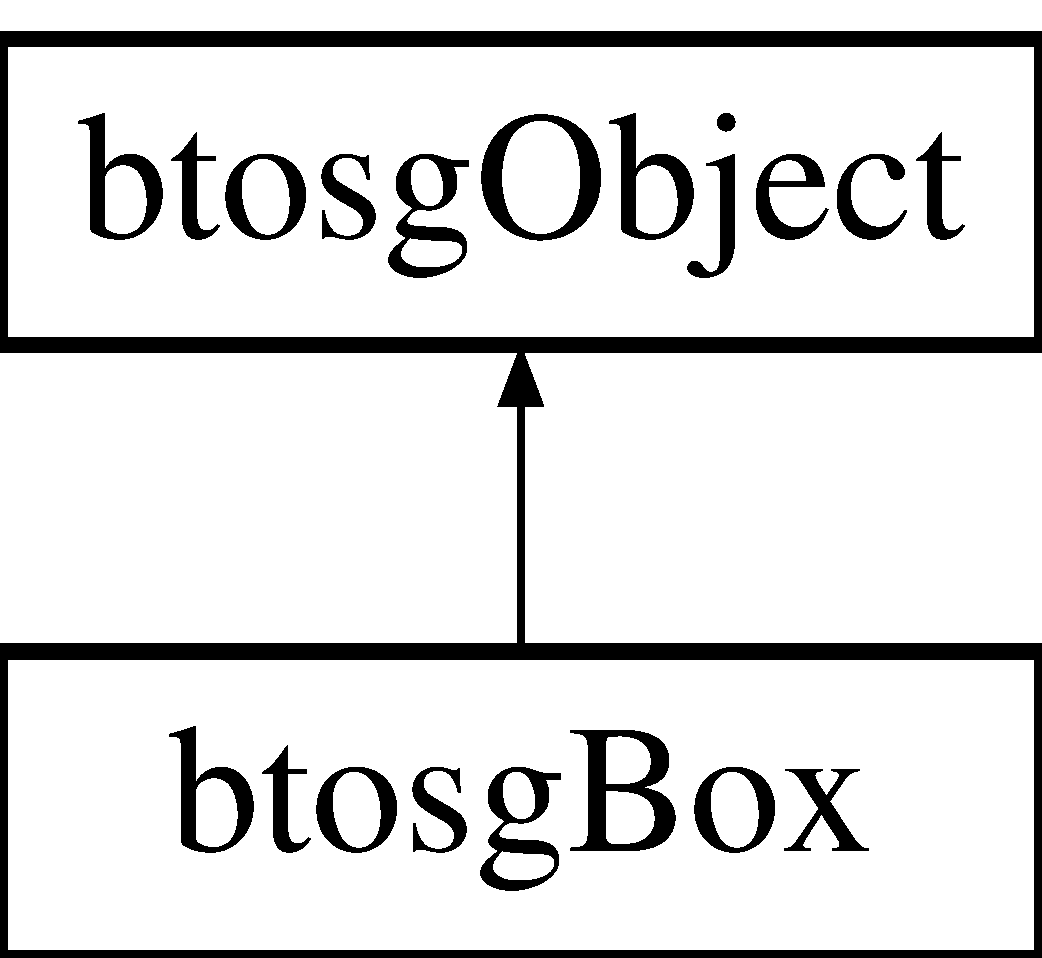
\includegraphics[height=2.000000cm]{classbtosgBox}
\end{center}
\end{figure}
\subsection*{Public Member Functions}
\begin{DoxyCompactItemize}
\item 
\hyperlink{classbtosgBox_aaffbdeeac3ee040dea98c19b538f0e49}{btosg\+Box} (\hyperlink{classbtosgVec3}{btosg\+Vec3} dim=\hyperlink{classbtosgVec3}{btosg\+Vec3}(1., 1., 1.), double m=1.)
\item 
\hyperlink{classbtosgBox_a0b7809cf498d50ced7c6e4a1bf0f5470}{btosg\+Box} (float x, float y, float z)
\item 
\hyperlink{classbtosgBox_a3b17e84e3f94aabdc7b8517bd802a5c9}{btosg\+Box} (float r)
\end{DoxyCompactItemize}
\subsection*{Public Attributes}
\begin{DoxyCompactItemize}
\item 
\mbox{\Hypertarget{classbtosgBox_a1d1e4744d9e377e1462ea097dacef716}\label{classbtosgBox_a1d1e4744d9e377e1462ea097dacef716}} 
float \hyperlink{classbtosgBox_a1d1e4744d9e377e1462ea097dacef716}{dx}
\begin{DoxyCompactList}\small\item\em x dimension \end{DoxyCompactList}\item 
\mbox{\Hypertarget{classbtosgBox_a7665337187adb52a1ce3b4cf2819217d}\label{classbtosgBox_a7665337187adb52a1ce3b4cf2819217d}} 
float \hyperlink{classbtosgBox_a7665337187adb52a1ce3b4cf2819217d}{dy}
\begin{DoxyCompactList}\small\item\em y dimension \end{DoxyCompactList}\item 
\mbox{\Hypertarget{classbtosgBox_a1dd905f6afb684d5d364f2b211dbab97}\label{classbtosgBox_a1dd905f6afb684d5d364f2b211dbab97}} 
float \hyperlink{classbtosgBox_a1dd905f6afb684d5d364f2b211dbab97}{dz}
\begin{DoxyCompactList}\small\item\em z dimension \end{DoxyCompactList}\end{DoxyCompactItemize}


\subsection{Detailed Description}
Axis oriented box. 

\subsection{Constructor \& Destructor Documentation}
\mbox{\Hypertarget{classbtosgBox_aaffbdeeac3ee040dea98c19b538f0e49}\label{classbtosgBox_aaffbdeeac3ee040dea98c19b538f0e49}} 
\index{btosg\+Box@{btosg\+Box}!btosg\+Box@{btosg\+Box}}
\index{btosg\+Box@{btosg\+Box}!btosg\+Box@{btosg\+Box}}
\subsubsection{\texorpdfstring{btosg\+Box()}{btosgBox()}\hspace{0.1cm}{\footnotesize\ttfamily [1/3]}}
{\footnotesize\ttfamily btosg\+Box\+::btosg\+Box (\begin{DoxyParamCaption}\item[{\hyperlink{classbtosgVec3}{btosg\+Vec3}}]{dim = {\ttfamily \hyperlink{classbtosgVec3}{btosg\+Vec3}(1.,1.,1.)},  }\item[{double}]{m = {\ttfamily 1.} }\end{DoxyParamCaption})\hspace{0.3cm}{\ttfamily [inline]}}

Constructs an axis oriented box. \mbox{\Hypertarget{classbtosgBox_a0b7809cf498d50ced7c6e4a1bf0f5470}\label{classbtosgBox_a0b7809cf498d50ced7c6e4a1bf0f5470}} 
\index{btosg\+Box@{btosg\+Box}!btosg\+Box@{btosg\+Box}}
\index{btosg\+Box@{btosg\+Box}!btosg\+Box@{btosg\+Box}}
\subsubsection{\texorpdfstring{btosg\+Box()}{btosgBox()}\hspace{0.1cm}{\footnotesize\ttfamily [2/3]}}
{\footnotesize\ttfamily btosg\+Box\+::btosg\+Box (\begin{DoxyParamCaption}\item[{float}]{x,  }\item[{float}]{y,  }\item[{float}]{z }\end{DoxyParamCaption})\hspace{0.3cm}{\ttfamily [inline]}}

Constructs an axis oriented box. \mbox{\Hypertarget{classbtosgBox_a3b17e84e3f94aabdc7b8517bd802a5c9}\label{classbtosgBox_a3b17e84e3f94aabdc7b8517bd802a5c9}} 
\index{btosg\+Box@{btosg\+Box}!btosg\+Box@{btosg\+Box}}
\index{btosg\+Box@{btosg\+Box}!btosg\+Box@{btosg\+Box}}
\subsubsection{\texorpdfstring{btosg\+Box()}{btosgBox()}\hspace{0.1cm}{\footnotesize\ttfamily [3/3]}}
{\footnotesize\ttfamily btosg\+Box\+::btosg\+Box (\begin{DoxyParamCaption}\item[{float}]{r }\end{DoxyParamCaption})\hspace{0.3cm}{\ttfamily [inline]}}

Constructs an axis oriented box. 

The documentation for this class was generated from the following file\+:\begin{DoxyCompactItemize}
\item 
btosg.\+h\end{DoxyCompactItemize}

\hypertarget{classbtosgCone}{}\section{btosg\+Cone Class Reference}
\label{classbtosgCone}\index{btosg\+Cone@{btosg\+Cone}}
Inheritance diagram for btosg\+Cone\+:\begin{figure}[H]
\begin{center}
\leavevmode
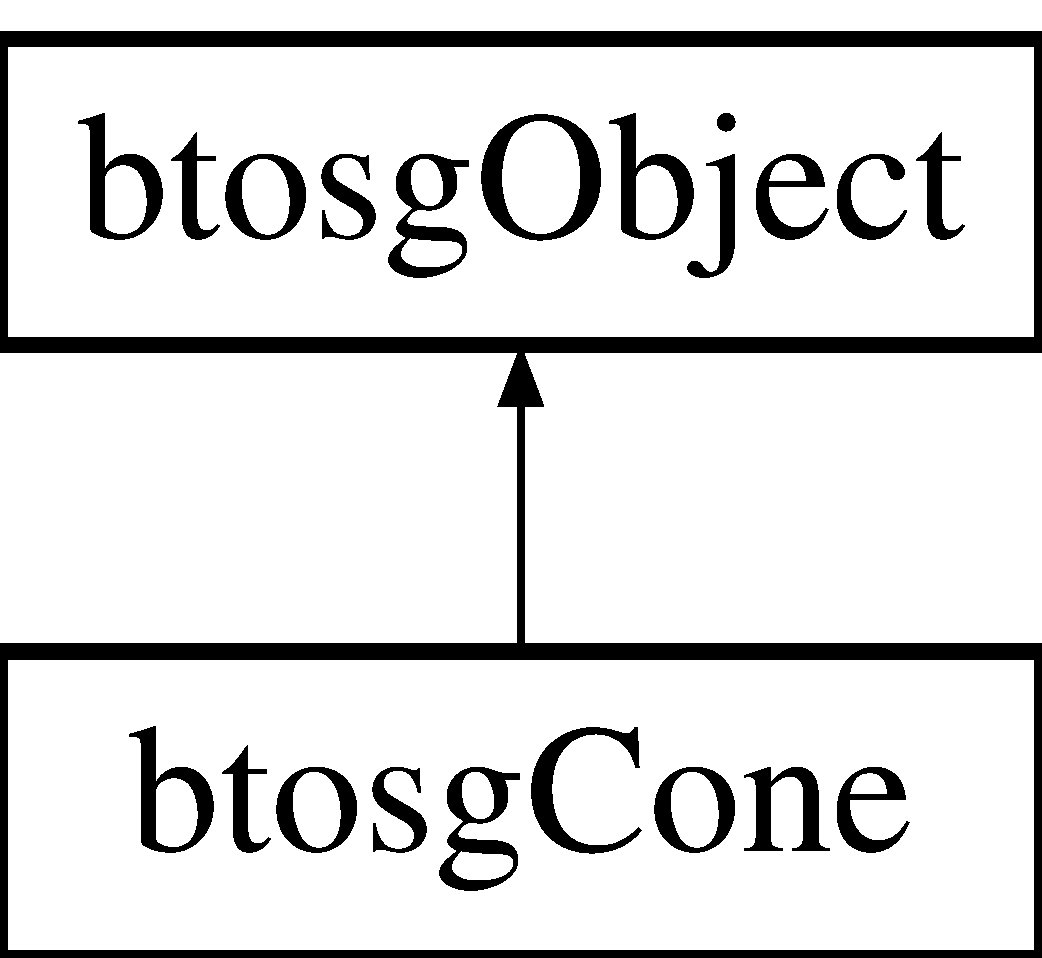
\includegraphics[height=2.000000cm]{classbtosgCone}
\end{center}
\end{figure}
\subsection*{Public Member Functions}
\begin{DoxyCompactItemize}
\item 
\mbox{\Hypertarget{classbtosgCone_a119bf79e2311ba084939d3e25086751c}\label{classbtosgCone_a119bf79e2311ba084939d3e25086751c}} 
{\bfseries btosg\+Cone} (float r=0.\+5, float h=1)
\end{DoxyCompactItemize}
\subsection*{Public Attributes}
\begin{DoxyCompactItemize}
\item 
\mbox{\Hypertarget{classbtosgCone_a75e351e13ad1e4d402f44a36838a6f4a}\label{classbtosgCone_a75e351e13ad1e4d402f44a36838a6f4a}} 
float {\bfseries radius}
\item 
\mbox{\Hypertarget{classbtosgCone_a1ddcbd82ff1fbaf69bc99d242819b83f}\label{classbtosgCone_a1ddcbd82ff1fbaf69bc99d242819b83f}} 
float {\bfseries height}
\end{DoxyCompactItemize}


The documentation for this class was generated from the following file\+:\begin{DoxyCompactItemize}
\item 
btosg.\+h\end{DoxyCompactItemize}

\hypertarget{classbtosgCylinder}{}\section{btosg\+Cylinder Class Reference}
\label{classbtosgCylinder}\index{btosg\+Cylinder@{btosg\+Cylinder}}


Cylinder.  




{\ttfamily \#include $<$btosg.\+h$>$}

Inheritance diagram for btosg\+Cylinder\+:\begin{figure}[H]
\begin{center}
\leavevmode
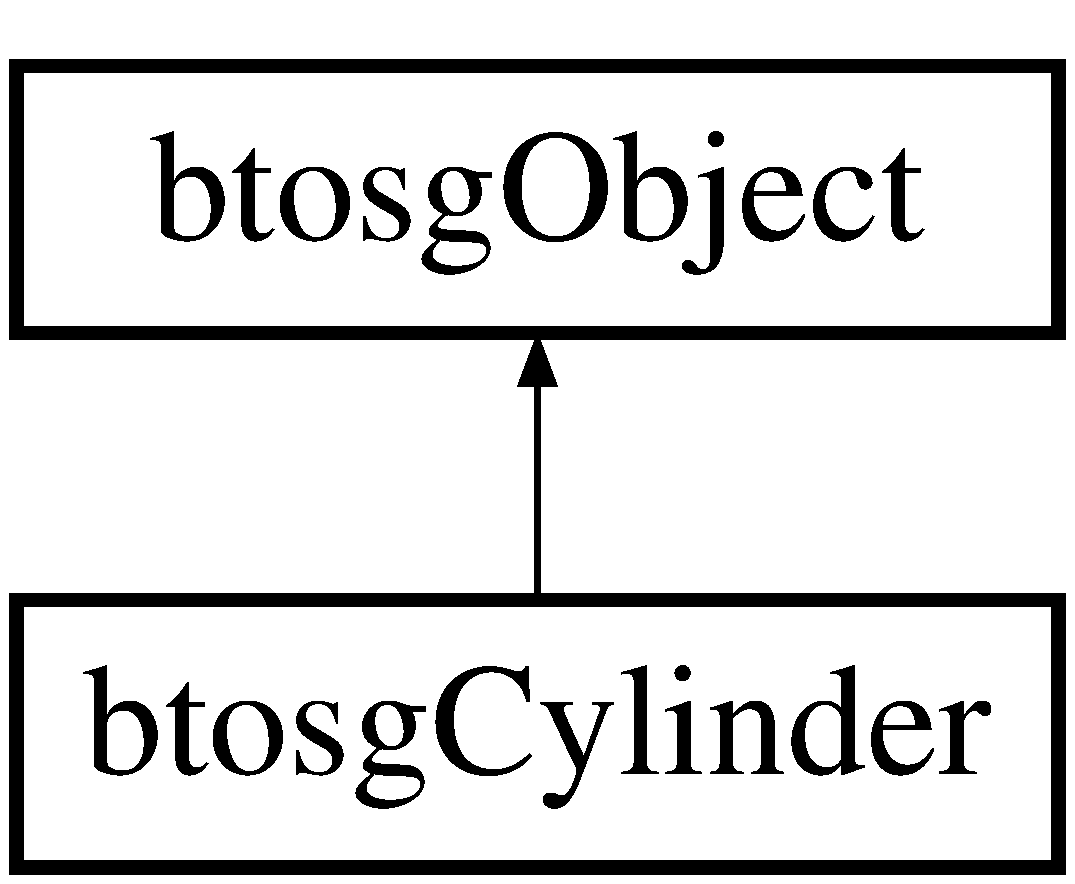
\includegraphics[height=2.000000cm]{classbtosgCylinder}
\end{center}
\end{figure}
\subsection*{Public Member Functions}
\begin{DoxyCompactItemize}
\item 
\hyperlink{classbtosgCylinder_a85e2517d8fd8a16ad7514f2f70cc1086}{btosg\+Cylinder} (float r=0.\+5, float h=1)
\item 
void \hyperlink{classbtosgObject_ab06a1b3f357209214c6440cd5746523e}{set\+Name} (char const $\ast$n)
\item 
void \hyperlink{classbtosgObject_a91da93c82d48b86192f0cbb16054fe57}{set\+Mass} (double m)
\item 
\hyperlink{classbtosgVec3}{btosg\+Vec3} \hyperlink{classbtosgObject_a3dadd5da8f2a312e44a039446b93d4cd}{get\+Position} ()
\item 
\hyperlink{classbtosgQuat}{btosg\+Quat} \hyperlink{classbtosgObject_a3b825999ad3a51bde743d4085ff19dae}{get\+Rotation} ()
\item 
\hyperlink{classbtosgVec3}{btosg\+Vec3} \hyperlink{classbtosgObject_a2019ec63bde02b72600450c7c985e77a}{get\+Euler} ()
\item 
void \hyperlink{classbtosgObject_ace6b51040b7ddce90818174200cc6074}{set\+Position} (const \hyperlink{classbtosgVec3}{btosg\+Vec3} \&p)
\item 
void \hyperlink{classbtosgObject_adb9f2cff0faf66dc252cd7c97b11ac84}{set\+Position} (float x, float y, float z)
\item 
void \hyperlink{classbtosgObject_a6365748d5506bb9da31907c9988071fa}{set\+Rotation} (\hyperlink{classbtosgQuat}{btosg\+Quat} q)
\item 
void \hyperlink{classbtosgObject_a4d21ca59b944fd26644db35d3e9ba67a}{set\+Rotation} (float x, float y, float z, float w)
\item 
void \hyperlink{classbtosgObject_aff54acbc7c66811efb0cf2838107a241}{set\+Texture} (char const $\ast$fname)
\item 
void \hyperlink{classbtosgObject_a6ab7b9e0553dab398b980637788b56a8}{set\+Material} (osg\+::ref\+\_\+ptr$<$ osg\+::\+Material $>$ mat)
\item 
void \hyperlink{classbtosgObject_acfd70fa6477c80fd7f29ad7ab9f4f067}{log\+Position} ()
\item 
virtual void \hyperlink{classbtosgObject_a342917817dfde62554f83da8e0d5110b}{update} ()
\item 
void \hyperlink{classbtosgObject_a93983f9180dd0672f8779cf2baa78580}{reset} ()
\item 
void \hyperlink{classbtosgObject_ad1508a0ce28cfac83e5f0ff6245f91b5}{set\+Init\+State} ()
\item 
void \hyperlink{classbtosgObject_a6ceb08e59ee95acaaef389ee198d2b56}{set\+Init\+State} (bt\+Transform i\+State)
\item 
void \hyperlink{classbtosgObject_a029dbe9134fa94e7355799f67fb2cd6d}{create\+Rigid\+Body} ()
\item 
void \hyperlink{classbtosgObject_a91838b8235579da178fcc06e6d3d47f3}{load\+Object\+Model} (char const $\ast$fname)
\end{DoxyCompactItemize}
\subsection*{Public Attributes}
\begin{DoxyCompactItemize}
\item 
\mbox{\Hypertarget{classbtosgObject_afd15726e7a214212d6d5815f8ac1ac6c}\label{classbtosgObject_afd15726e7a214212d6d5815f8ac1ac6c}} 
osg\+::ref\+\_\+ptr$<$ osg\+::\+Position\+Attitude\+Transform $>$ \hyperlink{classbtosgObject_afd15726e7a214212d6d5815f8ac1ac6c}{model}
\begin{DoxyCompactList}\small\item\em Object\textquotesingle{}s graphical model. \end{DoxyCompactList}\item 
\mbox{\Hypertarget{classbtosgObject_a12396e1362797a75473a2e833b579cc9}\label{classbtosgObject_a12396e1362797a75473a2e833b579cc9}} 
char $\ast$ \hyperlink{classbtosgObject_a12396e1362797a75473a2e833b579cc9}{name}
\begin{DoxyCompactList}\small\item\em Object name. \end{DoxyCompactList}\item 
\mbox{\Hypertarget{classbtosgObject_a2dee023f311114e200df9b04c8c1b400}\label{classbtosgObject_a2dee023f311114e200df9b04c8c1b400}} 
bt\+Transform \hyperlink{classbtosgObject_a2dee023f311114e200df9b04c8c1b400}{init\+\_\+state}
\begin{DoxyCompactList}\small\item\em Inital state. Applied on reset events. \end{DoxyCompactList}\item 
\mbox{\Hypertarget{classbtosgObject_a64ccde0543c184ed1749fdb9c9699785}\label{classbtosgObject_a64ccde0543c184ed1749fdb9c9699785}} 
bt\+Rigid\+Body $\ast$ \hyperlink{classbtosgObject_a64ccde0543c184ed1749fdb9c9699785}{body}
\begin{DoxyCompactList}\small\item\em object\textquotesingle{}s rigid body \end{DoxyCompactList}\item 
\mbox{\Hypertarget{classbtosgObject_a0f6a8da01cf643c321bffe86e42604b0}\label{classbtosgObject_a0f6a8da01cf643c321bffe86e42604b0}} 
bt\+Collision\+Shape $\ast$ \hyperlink{classbtosgObject_a0f6a8da01cf643c321bffe86e42604b0}{shape}
\begin{DoxyCompactList}\small\item\em Object\textquotesingle{}s collision shape. \end{DoxyCompactList}\item 
\mbox{\Hypertarget{classbtosgObject_a2418bb2194d5e9b0f1c51c84672ba7d1}\label{classbtosgObject_a2418bb2194d5e9b0f1c51c84672ba7d1}} 
float \hyperlink{classbtosgObject_a2418bb2194d5e9b0f1c51c84672ba7d1}{mass}
\begin{DoxyCompactList}\small\item\em Mass of object. \end{DoxyCompactList}\end{DoxyCompactItemize}


\subsection{Detailed Description}
Cylinder. 

\subsection{Constructor \& Destructor Documentation}
\mbox{\Hypertarget{classbtosgCylinder_a85e2517d8fd8a16ad7514f2f70cc1086}\label{classbtosgCylinder_a85e2517d8fd8a16ad7514f2f70cc1086}} 
\index{btosg\+Cylinder@{btosg\+Cylinder}!btosg\+Cylinder@{btosg\+Cylinder}}
\index{btosg\+Cylinder@{btosg\+Cylinder}!btosg\+Cylinder@{btosg\+Cylinder}}
\subsubsection{\texorpdfstring{btosg\+Cylinder()}{btosgCylinder()}}
{\footnotesize\ttfamily btosg\+Cylinder\+::btosg\+Cylinder (\begin{DoxyParamCaption}\item[{float}]{r = {\ttfamily 0.5},  }\item[{float}]{h = {\ttfamily 1} }\end{DoxyParamCaption})\hspace{0.3cm}{\ttfamily [inline]}}

Constructs a Z axis cylinder. 

\subsection{Member Function Documentation}
\mbox{\Hypertarget{classbtosgObject_a029dbe9134fa94e7355799f67fb2cd6d}\label{classbtosgObject_a029dbe9134fa94e7355799f67fb2cd6d}} 
\index{btosg\+Cylinder@{btosg\+Cylinder}!create\+Rigid\+Body@{create\+Rigid\+Body}}
\index{create\+Rigid\+Body@{create\+Rigid\+Body}!btosg\+Cylinder@{btosg\+Cylinder}}
\subsubsection{\texorpdfstring{create\+Rigid\+Body()}{createRigidBody()}}
{\footnotesize\ttfamily void btosg\+Object\+::create\+Rigid\+Body (\begin{DoxyParamCaption}{ }\end{DoxyParamCaption})\hspace{0.3cm}{\ttfamily [inline]}, {\ttfamily [inherited]}}

Creates a new rigid body as a bt\+Rigid\+Body object. \mbox{\Hypertarget{classbtosgObject_a2019ec63bde02b72600450c7c985e77a}\label{classbtosgObject_a2019ec63bde02b72600450c7c985e77a}} 
\index{btosg\+Cylinder@{btosg\+Cylinder}!get\+Euler@{get\+Euler}}
\index{get\+Euler@{get\+Euler}!btosg\+Cylinder@{btosg\+Cylinder}}
\subsubsection{\texorpdfstring{get\+Euler()}{getEuler()}}
{\footnotesize\ttfamily \hyperlink{classbtosgVec3}{btosg\+Vec3} btosg\+Object\+::get\+Euler (\begin{DoxyParamCaption}{ }\end{DoxyParamCaption})\hspace{0.3cm}{\ttfamily [inline]}, {\ttfamily [inherited]}}

Returns object\textquotesingle{}s attitude as H\+PR Euler angles. \mbox{\Hypertarget{classbtosgObject_a3dadd5da8f2a312e44a039446b93d4cd}\label{classbtosgObject_a3dadd5da8f2a312e44a039446b93d4cd}} 
\index{btosg\+Cylinder@{btosg\+Cylinder}!get\+Position@{get\+Position}}
\index{get\+Position@{get\+Position}!btosg\+Cylinder@{btosg\+Cylinder}}
\subsubsection{\texorpdfstring{get\+Position()}{getPosition()}}
{\footnotesize\ttfamily \hyperlink{classbtosgVec3}{btosg\+Vec3} btosg\+Object\+::get\+Position (\begin{DoxyParamCaption}{ }\end{DoxyParamCaption})\hspace{0.3cm}{\ttfamily [inline]}, {\ttfamily [inherited]}}

Returns object\textquotesingle{}s position. \mbox{\Hypertarget{classbtosgObject_a3b825999ad3a51bde743d4085ff19dae}\label{classbtosgObject_a3b825999ad3a51bde743d4085ff19dae}} 
\index{btosg\+Cylinder@{btosg\+Cylinder}!get\+Rotation@{get\+Rotation}}
\index{get\+Rotation@{get\+Rotation}!btosg\+Cylinder@{btosg\+Cylinder}}
\subsubsection{\texorpdfstring{get\+Rotation()}{getRotation()}}
{\footnotesize\ttfamily \hyperlink{classbtosgQuat}{btosg\+Quat} btosg\+Object\+::get\+Rotation (\begin{DoxyParamCaption}{ }\end{DoxyParamCaption})\hspace{0.3cm}{\ttfamily [inline]}, {\ttfamily [inherited]}}

Returns object\textquotesingle{}s attitude as a Quaternion. \mbox{\Hypertarget{classbtosgObject_a91838b8235579da178fcc06e6d3d47f3}\label{classbtosgObject_a91838b8235579da178fcc06e6d3d47f3}} 
\index{btosg\+Cylinder@{btosg\+Cylinder}!load\+Object\+Model@{load\+Object\+Model}}
\index{load\+Object\+Model@{load\+Object\+Model}!btosg\+Cylinder@{btosg\+Cylinder}}
\subsubsection{\texorpdfstring{load\+Object\+Model()}{loadObjectModel()}}
{\footnotesize\ttfamily void btosg\+Object\+::load\+Object\+Model (\begin{DoxyParamCaption}\item[{char const $\ast$}]{fname }\end{DoxyParamCaption})\hspace{0.3cm}{\ttfamily [inherited]}}

Loads an object model from a Wavefront O\+BJ file. Loadded model is used to define both the collision and graphical shapes. \mbox{\Hypertarget{classbtosgObject_acfd70fa6477c80fd7f29ad7ab9f4f067}\label{classbtosgObject_acfd70fa6477c80fd7f29ad7ab9f4f067}} 
\index{btosg\+Cylinder@{btosg\+Cylinder}!log\+Position@{log\+Position}}
\index{log\+Position@{log\+Position}!btosg\+Cylinder@{btosg\+Cylinder}}
\subsubsection{\texorpdfstring{log\+Position()}{logPosition()}}
{\footnotesize\ttfamily void btosg\+Object\+::log\+Position (\begin{DoxyParamCaption}{ }\end{DoxyParamCaption})\hspace{0.3cm}{\ttfamily [inline]}, {\ttfamily [inherited]}}

Outputs object\textquotesingle{}s position. \mbox{\Hypertarget{classbtosgObject_a93983f9180dd0672f8779cf2baa78580}\label{classbtosgObject_a93983f9180dd0672f8779cf2baa78580}} 
\index{btosg\+Cylinder@{btosg\+Cylinder}!reset@{reset}}
\index{reset@{reset}!btosg\+Cylinder@{btosg\+Cylinder}}
\subsubsection{\texorpdfstring{reset()}{reset()}}
{\footnotesize\ttfamily void btosg\+Object\+::reset (\begin{DoxyParamCaption}{ }\end{DoxyParamCaption})\hspace{0.3cm}{\ttfamily [inline]}, {\ttfamily [inherited]}}

Reposition object to its inital state. \mbox{\Hypertarget{classbtosgObject_ad1508a0ce28cfac83e5f0ff6245f91b5}\label{classbtosgObject_ad1508a0ce28cfac83e5f0ff6245f91b5}} 
\index{btosg\+Cylinder@{btosg\+Cylinder}!set\+Init\+State@{set\+Init\+State}}
\index{set\+Init\+State@{set\+Init\+State}!btosg\+Cylinder@{btosg\+Cylinder}}
\subsubsection{\texorpdfstring{set\+Init\+State()}{setInitState()}\hspace{0.1cm}{\footnotesize\ttfamily [1/2]}}
{\footnotesize\ttfamily void btosg\+Object\+::set\+Init\+State (\begin{DoxyParamCaption}{ }\end{DoxyParamCaption})\hspace{0.3cm}{\ttfamily [inline]}, {\ttfamily [inherited]}}

Stores current state as init state. Init state is aplied by \hyperlink{classbtosgObject_a93983f9180dd0672f8779cf2baa78580}{reset()} \mbox{\Hypertarget{classbtosgObject_a6ceb08e59ee95acaaef389ee198d2b56}\label{classbtosgObject_a6ceb08e59ee95acaaef389ee198d2b56}} 
\index{btosg\+Cylinder@{btosg\+Cylinder}!set\+Init\+State@{set\+Init\+State}}
\index{set\+Init\+State@{set\+Init\+State}!btosg\+Cylinder@{btosg\+Cylinder}}
\subsubsection{\texorpdfstring{set\+Init\+State()}{setInitState()}\hspace{0.1cm}{\footnotesize\ttfamily [2/2]}}
{\footnotesize\ttfamily void btosg\+Object\+::set\+Init\+State (\begin{DoxyParamCaption}\item[{bt\+Transform}]{i\+State }\end{DoxyParamCaption})\hspace{0.3cm}{\ttfamily [inline]}, {\ttfamily [inherited]}}

Stores i\+State as init state. Init state is aplied by \hyperlink{classbtosgObject_a93983f9180dd0672f8779cf2baa78580}{reset()} \mbox{\Hypertarget{classbtosgObject_a91da93c82d48b86192f0cbb16054fe57}\label{classbtosgObject_a91da93c82d48b86192f0cbb16054fe57}} 
\index{btosg\+Cylinder@{btosg\+Cylinder}!set\+Mass@{set\+Mass}}
\index{set\+Mass@{set\+Mass}!btosg\+Cylinder@{btosg\+Cylinder}}
\subsubsection{\texorpdfstring{set\+Mass()}{setMass()}}
{\footnotesize\ttfamily void btosg\+Object\+::set\+Mass (\begin{DoxyParamCaption}\item[{double}]{m }\end{DoxyParamCaption})\hspace{0.3cm}{\ttfamily [inline]}, {\ttfamily [inherited]}}

Sets the object\textquotesingle{}s mass. \mbox{\Hypertarget{classbtosgObject_a6ab7b9e0553dab398b980637788b56a8}\label{classbtosgObject_a6ab7b9e0553dab398b980637788b56a8}} 
\index{btosg\+Cylinder@{btosg\+Cylinder}!set\+Material@{set\+Material}}
\index{set\+Material@{set\+Material}!btosg\+Cylinder@{btosg\+Cylinder}}
\subsubsection{\texorpdfstring{set\+Material()}{setMaterial()}}
{\footnotesize\ttfamily void btosg\+Object\+::set\+Material (\begin{DoxyParamCaption}\item[{osg\+::ref\+\_\+ptr$<$ osg\+::\+Material $>$}]{mat }\end{DoxyParamCaption})\hspace{0.3cm}{\ttfamily [inline]}, {\ttfamily [inherited]}}

Sets the material properties for the object. \mbox{\Hypertarget{classbtosgObject_ab06a1b3f357209214c6440cd5746523e}\label{classbtosgObject_ab06a1b3f357209214c6440cd5746523e}} 
\index{btosg\+Cylinder@{btosg\+Cylinder}!set\+Name@{set\+Name}}
\index{set\+Name@{set\+Name}!btosg\+Cylinder@{btosg\+Cylinder}}
\subsubsection{\texorpdfstring{set\+Name()}{setName()}}
{\footnotesize\ttfamily void btosg\+Object\+::set\+Name (\begin{DoxyParamCaption}\item[{char const $\ast$}]{n }\end{DoxyParamCaption})\hspace{0.3cm}{\ttfamily [inline]}, {\ttfamily [inherited]}}

Sets the object\textquotesingle{}s name. \mbox{\Hypertarget{classbtosgObject_ace6b51040b7ddce90818174200cc6074}\label{classbtosgObject_ace6b51040b7ddce90818174200cc6074}} 
\index{btosg\+Cylinder@{btosg\+Cylinder}!set\+Position@{set\+Position}}
\index{set\+Position@{set\+Position}!btosg\+Cylinder@{btosg\+Cylinder}}
\subsubsection{\texorpdfstring{set\+Position()}{setPosition()}\hspace{0.1cm}{\footnotesize\ttfamily [1/2]}}
{\footnotesize\ttfamily void btosg\+Object\+::set\+Position (\begin{DoxyParamCaption}\item[{const \hyperlink{classbtosgVec3}{btosg\+Vec3} \&}]{p }\end{DoxyParamCaption})\hspace{0.3cm}{\ttfamily [inline]}, {\ttfamily [inherited]}}

Sets objects position. \mbox{\Hypertarget{classbtosgObject_adb9f2cff0faf66dc252cd7c97b11ac84}\label{classbtosgObject_adb9f2cff0faf66dc252cd7c97b11ac84}} 
\index{btosg\+Cylinder@{btosg\+Cylinder}!set\+Position@{set\+Position}}
\index{set\+Position@{set\+Position}!btosg\+Cylinder@{btosg\+Cylinder}}
\subsubsection{\texorpdfstring{set\+Position()}{setPosition()}\hspace{0.1cm}{\footnotesize\ttfamily [2/2]}}
{\footnotesize\ttfamily void btosg\+Object\+::set\+Position (\begin{DoxyParamCaption}\item[{float}]{x,  }\item[{float}]{y,  }\item[{float}]{z }\end{DoxyParamCaption})\hspace{0.3cm}{\ttfamily [inline]}, {\ttfamily [inherited]}}

Sets objects position. \mbox{\Hypertarget{classbtosgObject_a6365748d5506bb9da31907c9988071fa}\label{classbtosgObject_a6365748d5506bb9da31907c9988071fa}} 
\index{btosg\+Cylinder@{btosg\+Cylinder}!set\+Rotation@{set\+Rotation}}
\index{set\+Rotation@{set\+Rotation}!btosg\+Cylinder@{btosg\+Cylinder}}
\subsubsection{\texorpdfstring{set\+Rotation()}{setRotation()}\hspace{0.1cm}{\footnotesize\ttfamily [1/2]}}
{\footnotesize\ttfamily void btosg\+Object\+::set\+Rotation (\begin{DoxyParamCaption}\item[{\hyperlink{classbtosgQuat}{btosg\+Quat}}]{q }\end{DoxyParamCaption})\hspace{0.3cm}{\ttfamily [inline]}, {\ttfamily [inherited]}}

Sets objects attitude from a quaternion. \mbox{\Hypertarget{classbtosgObject_a4d21ca59b944fd26644db35d3e9ba67a}\label{classbtosgObject_a4d21ca59b944fd26644db35d3e9ba67a}} 
\index{btosg\+Cylinder@{btosg\+Cylinder}!set\+Rotation@{set\+Rotation}}
\index{set\+Rotation@{set\+Rotation}!btosg\+Cylinder@{btosg\+Cylinder}}
\subsubsection{\texorpdfstring{set\+Rotation()}{setRotation()}\hspace{0.1cm}{\footnotesize\ttfamily [2/2]}}
{\footnotesize\ttfamily void btosg\+Object\+::set\+Rotation (\begin{DoxyParamCaption}\item[{float}]{x,  }\item[{float}]{y,  }\item[{float}]{z,  }\item[{float}]{w }\end{DoxyParamCaption})\hspace{0.3cm}{\ttfamily [inline]}, {\ttfamily [inherited]}}

Sets objects attitude from the quaternion coords. \mbox{\Hypertarget{classbtosgObject_aff54acbc7c66811efb0cf2838107a241}\label{classbtosgObject_aff54acbc7c66811efb0cf2838107a241}} 
\index{btosg\+Cylinder@{btosg\+Cylinder}!set\+Texture@{set\+Texture}}
\index{set\+Texture@{set\+Texture}!btosg\+Cylinder@{btosg\+Cylinder}}
\subsubsection{\texorpdfstring{set\+Texture()}{setTexture()}}
{\footnotesize\ttfamily void btosg\+Object\+::set\+Texture (\begin{DoxyParamCaption}\item[{char const $\ast$}]{fname }\end{DoxyParamCaption})\hspace{0.3cm}{\ttfamily [inherited]}}

Sets the object texture from a loaded image file. \mbox{\Hypertarget{classbtosgObject_a342917817dfde62554f83da8e0d5110b}\label{classbtosgObject_a342917817dfde62554f83da8e0d5110b}} 
\index{btosg\+Cylinder@{btosg\+Cylinder}!update@{update}}
\index{update@{update}!btosg\+Cylinder@{btosg\+Cylinder}}
\subsubsection{\texorpdfstring{update()}{update()}}
{\footnotesize\ttfamily virtual void btosg\+Object\+::update (\begin{DoxyParamCaption}{ }\end{DoxyParamCaption})\hspace{0.3cm}{\ttfamily [inline]}, {\ttfamily [virtual]}, {\ttfamily [inherited]}}

Objects\textquotesingle{}s update callback. This function is called automatically from World\+::setp\+Simulation() for each registered object. Positions graphical object from its physhical state. 

Reimplemented in \hyperlink{classbtosgVehicle_a5fd0f471df492ac232c9b772a28bd2b9}{btosg\+Vehicle}.



The documentation for this class was generated from the following file\+:\begin{DoxyCompactItemize}
\item 
btosg.\+h\end{DoxyCompactItemize}

\hypertarget{classbtosgHUD}{}\section{btosg\+H\+UD Class Reference}
\label{classbtosgHUD}\index{btosgHUD@{btosgHUD}}


Head Up Display.  




{\ttfamily \#include $<$btosg\+H\+U\+D.\+h$>$}

Inheritance diagram for btosg\+H\+UD\+:\begin{figure}[H]
\begin{center}
\leavevmode
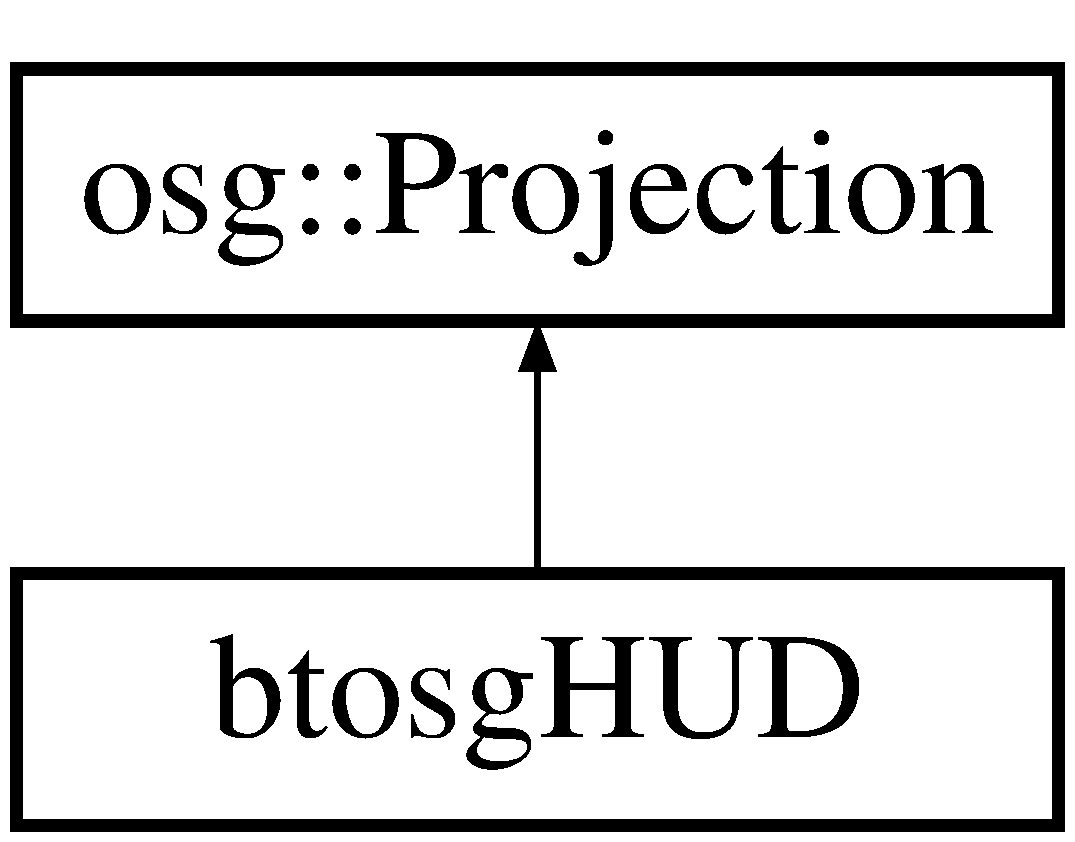
\includegraphics[height=2.000000cm]{classbtosgHUD}
\end{center}
\end{figure}
\subsection*{Public Member Functions}
\begin{DoxyCompactItemize}
\item 
void \mbox{\hyperlink{classbtosgHUD_a18c1eb80934574e6bdabbbee43e0bfeb}{set\+Background}} ()
\item 
\mbox{\hyperlink{classbtosgHUD_a1aee59dc4eff398996632f1e4b3e70fd}{btosg\+H\+UD}} ()
\item 
virtual bool \mbox{\hyperlink{classbtosgHUD_a182be3e4bdf00f9ff2b9c482833089a4}{add\+Drawable}} (osg\+::\+Drawable $\ast$td)
\end{DoxyCompactItemize}


\subsection{Detailed Description}
Head Up Display. 

\subsection{Constructor \& Destructor Documentation}
\mbox{\Hypertarget{classbtosgHUD_a1aee59dc4eff398996632f1e4b3e70fd}\label{classbtosgHUD_a1aee59dc4eff398996632f1e4b3e70fd}} 
\index{btosgHUD@{btosgHUD}!btosgHUD@{btosgHUD}}
\index{btosgHUD@{btosgHUD}!btosgHUD@{btosgHUD}}
\subsubsection{\texorpdfstring{btosgHUD()}{btosgHUD()}}
{\footnotesize\ttfamily btosg\+H\+U\+D\+::btosg\+H\+UD (\begin{DoxyParamCaption}{ }\end{DoxyParamCaption})\hspace{0.3cm}{\ttfamily [inline]}}

Constructs an Head Up Display. 

\subsection{Member Function Documentation}
\mbox{\Hypertarget{classbtosgHUD_a182be3e4bdf00f9ff2b9c482833089a4}\label{classbtosgHUD_a182be3e4bdf00f9ff2b9c482833089a4}} 
\index{btosgHUD@{btosgHUD}!addDrawable@{addDrawable}}
\index{addDrawable@{addDrawable}!btosgHUD@{btosgHUD}}
\subsubsection{\texorpdfstring{addDrawable()}{addDrawable()}}
{\footnotesize\ttfamily virtual bool btosg\+H\+U\+D\+::add\+Drawable (\begin{DoxyParamCaption}\item[{osg\+::\+Drawable $\ast$}]{td }\end{DoxyParamCaption})\hspace{0.3cm}{\ttfamily [inline]}, {\ttfamily [virtual]}}

Add a visual elemente to the H\+UD. \mbox{\Hypertarget{classbtosgHUD_a18c1eb80934574e6bdabbbee43e0bfeb}\label{classbtosgHUD_a18c1eb80934574e6bdabbbee43e0bfeb}} 
\index{btosgHUD@{btosgHUD}!setBackground@{setBackground}}
\index{setBackground@{setBackground}!btosgHUD@{btosgHUD}}
\subsubsection{\texorpdfstring{setBackground()}{setBackground()}}
{\footnotesize\ttfamily void btosg\+H\+U\+D\+::set\+Background (\begin{DoxyParamCaption}{ }\end{DoxyParamCaption})\hspace{0.3cm}{\ttfamily [inline]}}

Set up geometry for the H\+UD and add it to the H\+UD 

The documentation for this class was generated from the following file\+:\begin{DoxyCompactItemize}
\item 
btosg\+H\+U\+D.\+h\end{DoxyCompactItemize}

\hypertarget{classbtosgObject}{}\section{btosg\+Object Class Reference}
\label{classbtosgObject}\index{btosg\+Object@{btosg\+Object}}


Main btosg object base class. Integrates a physical object (bt\+Rigid\+Body), a collision shape (bt\+Collision\+Shape) and a graphical object (osg\+::\+Position\+Attitude\+Transform).  




{\ttfamily \#include $<$btosg.\+h$>$}

Inheritance diagram for btosg\+Object\+:\begin{figure}[H]
\begin{center}
\leavevmode
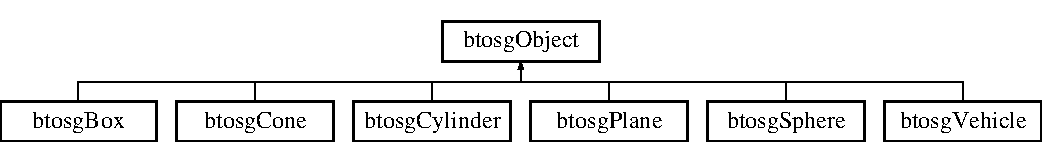
\includegraphics[height=1.904762cm]{classbtosgObject}
\end{center}
\end{figure}
\subsection*{Public Member Functions}
\begin{DoxyCompactItemize}
\item 
void \hyperlink{classbtosgObject_ab06a1b3f357209214c6440cd5746523e}{set\+Name} (char const $\ast$n)
\item 
void \hyperlink{classbtosgObject_a91da93c82d48b86192f0cbb16054fe57}{set\+Mass} (double m)
\item 
bt\+Vector3 \hyperlink{classbtosgObject_a77a1434498d7a6d00c415042a995d119}{get\+Position} ()
\item 
bt\+Quaternion \hyperlink{classbtosgObject_a9cadb03762699412552601196950a039}{get\+Rotation} ()
\item 
bt\+Vector3 \hyperlink{classbtosgObject_afef1fe06635566ab9cee134f72439e02}{get\+Euler} ()
\item 
void \hyperlink{classbtosgObject_ad0f76df8e8bde6c8a9d1b1d53551172b}{set\+Position} (const bt\+Vector3 \&p)
\item 
void \hyperlink{classbtosgObject_adb9f2cff0faf66dc252cd7c97b11ac84}{set\+Position} (float x, float y, float z)
\item 
void \hyperlink{classbtosgObject_a656412794a971a10478aedb520f298bf}{set\+Rotation} (bt\+Quaternion q)
\item 
void \hyperlink{classbtosgObject_a4d21ca59b944fd26644db35d3e9ba67a}{set\+Rotation} (float x, float y, float z, float w)
\item 
void \hyperlink{classbtosgObject_ae803e0566f0d7b3ffca686b968b297f8}{set\+Rotation} (osg\+::\+Quat q)
\item 
void \hyperlink{classbtosgObject_aff54acbc7c66811efb0cf2838107a241}{set\+Texture} (char const $\ast$fname)
\item 
void \hyperlink{classbtosgObject_a6ab7b9e0553dab398b980637788b56a8}{set\+Material} (osg\+::ref\+\_\+ptr$<$ osg\+::\+Material $>$ mat)
\item 
void \hyperlink{classbtosgObject_acfd70fa6477c80fd7f29ad7ab9f4f067}{log\+Position} ()
\item 
virtual void \hyperlink{classbtosgObject_a342917817dfde62554f83da8e0d5110b}{update} ()
\item 
void \hyperlink{classbtosgObject_a93983f9180dd0672f8779cf2baa78580}{reset} ()
\item 
void \hyperlink{classbtosgObject_ad1508a0ce28cfac83e5f0ff6245f91b5}{set\+Init\+State} ()
\item 
void \hyperlink{classbtosgObject_a6ceb08e59ee95acaaef389ee198d2b56}{set\+Init\+State} (bt\+Transform i\+State)
\item 
void \hyperlink{classbtosgObject_a029dbe9134fa94e7355799f67fb2cd6d}{create\+Rigid\+Body} ()
\item 
void \hyperlink{classbtosgObject_a91838b8235579da178fcc06e6d3d47f3}{load\+Object\+Model} (char const $\ast$fname)
\end{DoxyCompactItemize}
\subsection*{Public Attributes}
\begin{DoxyCompactItemize}
\item 
\mbox{\Hypertarget{classbtosgObject_afd15726e7a214212d6d5815f8ac1ac6c}\label{classbtosgObject_afd15726e7a214212d6d5815f8ac1ac6c}} 
osg\+::ref\+\_\+ptr$<$ osg\+::\+Position\+Attitude\+Transform $>$ \hyperlink{classbtosgObject_afd15726e7a214212d6d5815f8ac1ac6c}{model}
\begin{DoxyCompactList}\small\item\em Object\textquotesingle{}s graphical model. \end{DoxyCompactList}\item 
\mbox{\Hypertarget{classbtosgObject_a12396e1362797a75473a2e833b579cc9}\label{classbtosgObject_a12396e1362797a75473a2e833b579cc9}} 
char $\ast$ \hyperlink{classbtosgObject_a12396e1362797a75473a2e833b579cc9}{name}
\begin{DoxyCompactList}\small\item\em Object name. \end{DoxyCompactList}\item 
\mbox{\Hypertarget{classbtosgObject_a2dee023f311114e200df9b04c8c1b400}\label{classbtosgObject_a2dee023f311114e200df9b04c8c1b400}} 
bt\+Transform \hyperlink{classbtosgObject_a2dee023f311114e200df9b04c8c1b400}{init\+\_\+state}
\begin{DoxyCompactList}\small\item\em Inital state. Applied on reset events. \end{DoxyCompactList}\item 
\mbox{\Hypertarget{classbtosgObject_a64ccde0543c184ed1749fdb9c9699785}\label{classbtosgObject_a64ccde0543c184ed1749fdb9c9699785}} 
bt\+Rigid\+Body $\ast$ \hyperlink{classbtosgObject_a64ccde0543c184ed1749fdb9c9699785}{body}
\begin{DoxyCompactList}\small\item\em object\textquotesingle{}s rigid body \end{DoxyCompactList}\item 
\mbox{\Hypertarget{classbtosgObject_a0f6a8da01cf643c321bffe86e42604b0}\label{classbtosgObject_a0f6a8da01cf643c321bffe86e42604b0}} 
bt\+Collision\+Shape $\ast$ \hyperlink{classbtosgObject_a0f6a8da01cf643c321bffe86e42604b0}{shape}
\begin{DoxyCompactList}\small\item\em Object\textquotesingle{}s collision shape. \end{DoxyCompactList}\item 
\mbox{\Hypertarget{classbtosgObject_a2418bb2194d5e9b0f1c51c84672ba7d1}\label{classbtosgObject_a2418bb2194d5e9b0f1c51c84672ba7d1}} 
float \hyperlink{classbtosgObject_a2418bb2194d5e9b0f1c51c84672ba7d1}{mass}
\begin{DoxyCompactList}\small\item\em Mass of object. \end{DoxyCompactList}\end{DoxyCompactItemize}


\subsection{Detailed Description}
Main btosg object base class. Integrates a physical object (bt\+Rigid\+Body), a collision shape (bt\+Collision\+Shape) and a graphical object (osg\+::\+Position\+Attitude\+Transform). 

\subsection{Member Function Documentation}
\mbox{\Hypertarget{classbtosgObject_a029dbe9134fa94e7355799f67fb2cd6d}\label{classbtosgObject_a029dbe9134fa94e7355799f67fb2cd6d}} 
\index{btosg\+Object@{btosg\+Object}!create\+Rigid\+Body@{create\+Rigid\+Body}}
\index{create\+Rigid\+Body@{create\+Rigid\+Body}!btosg\+Object@{btosg\+Object}}
\subsubsection{\texorpdfstring{create\+Rigid\+Body()}{createRigidBody()}}
{\footnotesize\ttfamily void btosg\+Object\+::create\+Rigid\+Body (\begin{DoxyParamCaption}{ }\end{DoxyParamCaption})\hspace{0.3cm}{\ttfamily [inline]}}

Creates a new rigid body as a bt\+Rigid\+Body object. \mbox{\Hypertarget{classbtosgObject_afef1fe06635566ab9cee134f72439e02}\label{classbtosgObject_afef1fe06635566ab9cee134f72439e02}} 
\index{btosg\+Object@{btosg\+Object}!get\+Euler@{get\+Euler}}
\index{get\+Euler@{get\+Euler}!btosg\+Object@{btosg\+Object}}
\subsubsection{\texorpdfstring{get\+Euler()}{getEuler()}}
{\footnotesize\ttfamily bt\+Vector3 btosg\+Object\+::get\+Euler (\begin{DoxyParamCaption}{ }\end{DoxyParamCaption})\hspace{0.3cm}{\ttfamily [inline]}}

Returns object\textquotesingle{}s attitude as H\+PR Euler angles. \mbox{\Hypertarget{classbtosgObject_a77a1434498d7a6d00c415042a995d119}\label{classbtosgObject_a77a1434498d7a6d00c415042a995d119}} 
\index{btosg\+Object@{btosg\+Object}!get\+Position@{get\+Position}}
\index{get\+Position@{get\+Position}!btosg\+Object@{btosg\+Object}}
\subsubsection{\texorpdfstring{get\+Position()}{getPosition()}}
{\footnotesize\ttfamily bt\+Vector3 btosg\+Object\+::get\+Position (\begin{DoxyParamCaption}{ }\end{DoxyParamCaption})\hspace{0.3cm}{\ttfamily [inline]}}

Returns object\textquotesingle{}s position. \mbox{\Hypertarget{classbtosgObject_a9cadb03762699412552601196950a039}\label{classbtosgObject_a9cadb03762699412552601196950a039}} 
\index{btosg\+Object@{btosg\+Object}!get\+Rotation@{get\+Rotation}}
\index{get\+Rotation@{get\+Rotation}!btosg\+Object@{btosg\+Object}}
\subsubsection{\texorpdfstring{get\+Rotation()}{getRotation()}}
{\footnotesize\ttfamily bt\+Quaternion btosg\+Object\+::get\+Rotation (\begin{DoxyParamCaption}{ }\end{DoxyParamCaption})\hspace{0.3cm}{\ttfamily [inline]}}

Returns object\textquotesingle{}s attitude as a Quaternion. \mbox{\Hypertarget{classbtosgObject_a91838b8235579da178fcc06e6d3d47f3}\label{classbtosgObject_a91838b8235579da178fcc06e6d3d47f3}} 
\index{btosg\+Object@{btosg\+Object}!load\+Object\+Model@{load\+Object\+Model}}
\index{load\+Object\+Model@{load\+Object\+Model}!btosg\+Object@{btosg\+Object}}
\subsubsection{\texorpdfstring{load\+Object\+Model()}{loadObjectModel()}}
{\footnotesize\ttfamily void btosg\+Object\+::load\+Object\+Model (\begin{DoxyParamCaption}\item[{char const $\ast$}]{fname }\end{DoxyParamCaption})}

Loads an object model from a Wavefront O\+BJ file. Loadded model is used to defne bith the collision and graphical shapes. \mbox{\Hypertarget{classbtosgObject_acfd70fa6477c80fd7f29ad7ab9f4f067}\label{classbtosgObject_acfd70fa6477c80fd7f29ad7ab9f4f067}} 
\index{btosg\+Object@{btosg\+Object}!log\+Position@{log\+Position}}
\index{log\+Position@{log\+Position}!btosg\+Object@{btosg\+Object}}
\subsubsection{\texorpdfstring{log\+Position()}{logPosition()}}
{\footnotesize\ttfamily void btosg\+Object\+::log\+Position (\begin{DoxyParamCaption}{ }\end{DoxyParamCaption})\hspace{0.3cm}{\ttfamily [inline]}}

Outputs object\textquotesingle{}s position. \mbox{\Hypertarget{classbtosgObject_a93983f9180dd0672f8779cf2baa78580}\label{classbtosgObject_a93983f9180dd0672f8779cf2baa78580}} 
\index{btosg\+Object@{btosg\+Object}!reset@{reset}}
\index{reset@{reset}!btosg\+Object@{btosg\+Object}}
\subsubsection{\texorpdfstring{reset()}{reset()}}
{\footnotesize\ttfamily void btosg\+Object\+::reset (\begin{DoxyParamCaption}{ }\end{DoxyParamCaption})\hspace{0.3cm}{\ttfamily [inline]}}

Reposition object to its inital state. \mbox{\Hypertarget{classbtosgObject_ad1508a0ce28cfac83e5f0ff6245f91b5}\label{classbtosgObject_ad1508a0ce28cfac83e5f0ff6245f91b5}} 
\index{btosg\+Object@{btosg\+Object}!set\+Init\+State@{set\+Init\+State}}
\index{set\+Init\+State@{set\+Init\+State}!btosg\+Object@{btosg\+Object}}
\subsubsection{\texorpdfstring{set\+Init\+State()}{setInitState()}\hspace{0.1cm}{\footnotesize\ttfamily [1/2]}}
{\footnotesize\ttfamily void btosg\+Object\+::set\+Init\+State (\begin{DoxyParamCaption}{ }\end{DoxyParamCaption})\hspace{0.3cm}{\ttfamily [inline]}}

Stores current state as init state. Init state is aplied by \hyperlink{classbtosgObject_a93983f9180dd0672f8779cf2baa78580}{reset()} \mbox{\Hypertarget{classbtosgObject_a6ceb08e59ee95acaaef389ee198d2b56}\label{classbtosgObject_a6ceb08e59ee95acaaef389ee198d2b56}} 
\index{btosg\+Object@{btosg\+Object}!set\+Init\+State@{set\+Init\+State}}
\index{set\+Init\+State@{set\+Init\+State}!btosg\+Object@{btosg\+Object}}
\subsubsection{\texorpdfstring{set\+Init\+State()}{setInitState()}\hspace{0.1cm}{\footnotesize\ttfamily [2/2]}}
{\footnotesize\ttfamily void btosg\+Object\+::set\+Init\+State (\begin{DoxyParamCaption}\item[{bt\+Transform}]{i\+State }\end{DoxyParamCaption})\hspace{0.3cm}{\ttfamily [inline]}}

Stores i\+State as init state. Init state is aplied by \hyperlink{classbtosgObject_a93983f9180dd0672f8779cf2baa78580}{reset()} \mbox{\Hypertarget{classbtosgObject_a91da93c82d48b86192f0cbb16054fe57}\label{classbtosgObject_a91da93c82d48b86192f0cbb16054fe57}} 
\index{btosg\+Object@{btosg\+Object}!set\+Mass@{set\+Mass}}
\index{set\+Mass@{set\+Mass}!btosg\+Object@{btosg\+Object}}
\subsubsection{\texorpdfstring{set\+Mass()}{setMass()}}
{\footnotesize\ttfamily void btosg\+Object\+::set\+Mass (\begin{DoxyParamCaption}\item[{double}]{m }\end{DoxyParamCaption})\hspace{0.3cm}{\ttfamily [inline]}}

Sets the object\textquotesingle{}s mass. \mbox{\Hypertarget{classbtosgObject_a6ab7b9e0553dab398b980637788b56a8}\label{classbtosgObject_a6ab7b9e0553dab398b980637788b56a8}} 
\index{btosg\+Object@{btosg\+Object}!set\+Material@{set\+Material}}
\index{set\+Material@{set\+Material}!btosg\+Object@{btosg\+Object}}
\subsubsection{\texorpdfstring{set\+Material()}{setMaterial()}}
{\footnotesize\ttfamily void btosg\+Object\+::set\+Material (\begin{DoxyParamCaption}\item[{osg\+::ref\+\_\+ptr$<$ osg\+::\+Material $>$}]{mat }\end{DoxyParamCaption})\hspace{0.3cm}{\ttfamily [inline]}}

Sets the material properties for the object. \mbox{\Hypertarget{classbtosgObject_ab06a1b3f357209214c6440cd5746523e}\label{classbtosgObject_ab06a1b3f357209214c6440cd5746523e}} 
\index{btosg\+Object@{btosg\+Object}!set\+Name@{set\+Name}}
\index{set\+Name@{set\+Name}!btosg\+Object@{btosg\+Object}}
\subsubsection{\texorpdfstring{set\+Name()}{setName()}}
{\footnotesize\ttfamily void btosg\+Object\+::set\+Name (\begin{DoxyParamCaption}\item[{char const $\ast$}]{n }\end{DoxyParamCaption})\hspace{0.3cm}{\ttfamily [inline]}}

Sets the object\textquotesingle{}s name. \mbox{\Hypertarget{classbtosgObject_ad0f76df8e8bde6c8a9d1b1d53551172b}\label{classbtosgObject_ad0f76df8e8bde6c8a9d1b1d53551172b}} 
\index{btosg\+Object@{btosg\+Object}!set\+Position@{set\+Position}}
\index{set\+Position@{set\+Position}!btosg\+Object@{btosg\+Object}}
\subsubsection{\texorpdfstring{set\+Position()}{setPosition()}\hspace{0.1cm}{\footnotesize\ttfamily [1/2]}}
{\footnotesize\ttfamily void btosg\+Object\+::set\+Position (\begin{DoxyParamCaption}\item[{const bt\+Vector3 \&}]{p }\end{DoxyParamCaption})\hspace{0.3cm}{\ttfamily [inline]}}

Sets objects position. \mbox{\Hypertarget{classbtosgObject_adb9f2cff0faf66dc252cd7c97b11ac84}\label{classbtosgObject_adb9f2cff0faf66dc252cd7c97b11ac84}} 
\index{btosg\+Object@{btosg\+Object}!set\+Position@{set\+Position}}
\index{set\+Position@{set\+Position}!btosg\+Object@{btosg\+Object}}
\subsubsection{\texorpdfstring{set\+Position()}{setPosition()}\hspace{0.1cm}{\footnotesize\ttfamily [2/2]}}
{\footnotesize\ttfamily void btosg\+Object\+::set\+Position (\begin{DoxyParamCaption}\item[{float}]{x,  }\item[{float}]{y,  }\item[{float}]{z }\end{DoxyParamCaption})\hspace{0.3cm}{\ttfamily [inline]}}

Sets objects position. \mbox{\Hypertarget{classbtosgObject_a656412794a971a10478aedb520f298bf}\label{classbtosgObject_a656412794a971a10478aedb520f298bf}} 
\index{btosg\+Object@{btosg\+Object}!set\+Rotation@{set\+Rotation}}
\index{set\+Rotation@{set\+Rotation}!btosg\+Object@{btosg\+Object}}
\subsubsection{\texorpdfstring{set\+Rotation()}{setRotation()}\hspace{0.1cm}{\footnotesize\ttfamily [1/3]}}
{\footnotesize\ttfamily void btosg\+Object\+::set\+Rotation (\begin{DoxyParamCaption}\item[{bt\+Quaternion}]{q }\end{DoxyParamCaption})\hspace{0.3cm}{\ttfamily [inline]}}

Sets objects attitude from a quaternion. \mbox{\Hypertarget{classbtosgObject_a4d21ca59b944fd26644db35d3e9ba67a}\label{classbtosgObject_a4d21ca59b944fd26644db35d3e9ba67a}} 
\index{btosg\+Object@{btosg\+Object}!set\+Rotation@{set\+Rotation}}
\index{set\+Rotation@{set\+Rotation}!btosg\+Object@{btosg\+Object}}
\subsubsection{\texorpdfstring{set\+Rotation()}{setRotation()}\hspace{0.1cm}{\footnotesize\ttfamily [2/3]}}
{\footnotesize\ttfamily void btosg\+Object\+::set\+Rotation (\begin{DoxyParamCaption}\item[{float}]{x,  }\item[{float}]{y,  }\item[{float}]{z,  }\item[{float}]{w }\end{DoxyParamCaption})\hspace{0.3cm}{\ttfamily [inline]}}

Sets objects attitude from the quaternion coords. \mbox{\Hypertarget{classbtosgObject_ae803e0566f0d7b3ffca686b968b297f8}\label{classbtosgObject_ae803e0566f0d7b3ffca686b968b297f8}} 
\index{btosg\+Object@{btosg\+Object}!set\+Rotation@{set\+Rotation}}
\index{set\+Rotation@{set\+Rotation}!btosg\+Object@{btosg\+Object}}
\subsubsection{\texorpdfstring{set\+Rotation()}{setRotation()}\hspace{0.1cm}{\footnotesize\ttfamily [3/3]}}
{\footnotesize\ttfamily void btosg\+Object\+::set\+Rotation (\begin{DoxyParamCaption}\item[{osg\+::\+Quat}]{q }\end{DoxyParamCaption})\hspace{0.3cm}{\ttfamily [inline]}}

Sets objects attitude from a quaternion. \mbox{\Hypertarget{classbtosgObject_aff54acbc7c66811efb0cf2838107a241}\label{classbtosgObject_aff54acbc7c66811efb0cf2838107a241}} 
\index{btosg\+Object@{btosg\+Object}!set\+Texture@{set\+Texture}}
\index{set\+Texture@{set\+Texture}!btosg\+Object@{btosg\+Object}}
\subsubsection{\texorpdfstring{set\+Texture()}{setTexture()}}
{\footnotesize\ttfamily void btosg\+Object\+::set\+Texture (\begin{DoxyParamCaption}\item[{char const $\ast$}]{fname }\end{DoxyParamCaption})}

Sets the object texture from a loaded image file. \mbox{\Hypertarget{classbtosgObject_a342917817dfde62554f83da8e0d5110b}\label{classbtosgObject_a342917817dfde62554f83da8e0d5110b}} 
\index{btosg\+Object@{btosg\+Object}!update@{update}}
\index{update@{update}!btosg\+Object@{btosg\+Object}}
\subsubsection{\texorpdfstring{update()}{update()}}
{\footnotesize\ttfamily virtual void btosg\+Object\+::update (\begin{DoxyParamCaption}{ }\end{DoxyParamCaption})\hspace{0.3cm}{\ttfamily [inline]}, {\ttfamily [virtual]}}

Objects\textquotesingle{}s update callback. This function is called automatically from World\+::setp\+Simulation() for each registered object. Positions graphical object from its physhical state. 

Reimplemented in \hyperlink{classbtosgVehicle_a5fd0f471df492ac232c9b772a28bd2b9}{btosg\+Vehicle}.



The documentation for this class was generated from the following files\+:\begin{DoxyCompactItemize}
\item 
btosg.\+h\item 
btosg.\+cpp\end{DoxyCompactItemize}

\hypertarget{classbtosgPlane}{}\section{btosg\+Plane Class Reference}
\label{classbtosgPlane}\index{btosg\+Plane@{btosg\+Plane}}


Infinite plane.  




{\ttfamily \#include $<$btosg.\+h$>$}

Inheritance diagram for btosg\+Plane\+:\begin{figure}[H]
\begin{center}
\leavevmode
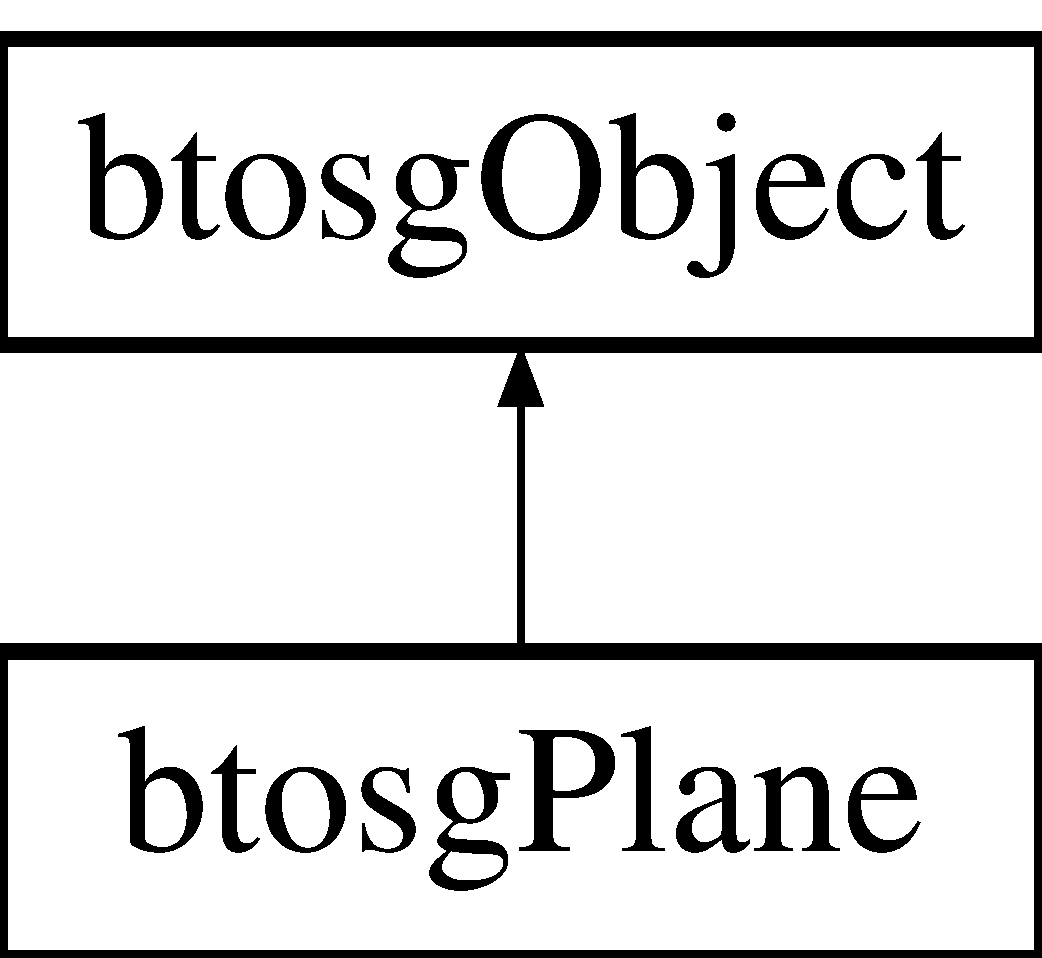
\includegraphics[height=2.000000cm]{classbtosgPlane}
\end{center}
\end{figure}
\subsection*{Public Member Functions}
\begin{DoxyCompactItemize}
\item 
\hyperlink{classbtosgPlane_a363737cea03a886470a1a46003706268}{btosg\+Plane} ()
\item 
\hyperlink{classbtosgPlane_a56b020a475b1c955fc50d5c1f6d4d754}{btosg\+Plane} (\hyperlink{classbtosgVec3}{btosg\+Vec3} v)
\item 
\hyperlink{classbtosgPlane_a295ebe4cb55a2786764c7840d10895f4}{btosg\+Plane} (float dx, float dy, float dz)
\item 
void \hyperlink{classbtosgPlane_a0e6812c186ed1fa128dccf7cd2e525a6}{create\+Rigid\+Body} ()
\item 
void \hyperlink{classbtosgObject_ab06a1b3f357209214c6440cd5746523e}{set\+Name} (char const $\ast$n)
\item 
void \hyperlink{classbtosgObject_a91da93c82d48b86192f0cbb16054fe57}{set\+Mass} (double m)
\item 
\hyperlink{classbtosgVec3}{btosg\+Vec3} \hyperlink{classbtosgObject_a3dadd5da8f2a312e44a039446b93d4cd}{get\+Position} ()
\item 
\hyperlink{classbtosgQuat}{btosg\+Quat} \hyperlink{classbtosgObject_a3b825999ad3a51bde743d4085ff19dae}{get\+Rotation} ()
\item 
\hyperlink{classbtosgVec3}{btosg\+Vec3} \hyperlink{classbtosgObject_a2019ec63bde02b72600450c7c985e77a}{get\+Euler} ()
\item 
void \hyperlink{classbtosgObject_ace6b51040b7ddce90818174200cc6074}{set\+Position} (const \hyperlink{classbtosgVec3}{btosg\+Vec3} \&p)
\item 
void \hyperlink{classbtosgObject_adb9f2cff0faf66dc252cd7c97b11ac84}{set\+Position} (float x, float y, float z)
\item 
void \hyperlink{classbtosgObject_a6365748d5506bb9da31907c9988071fa}{set\+Rotation} (\hyperlink{classbtosgQuat}{btosg\+Quat} q)
\item 
void \hyperlink{classbtosgObject_a4d21ca59b944fd26644db35d3e9ba67a}{set\+Rotation} (float x, float y, float z, float w)
\item 
void \hyperlink{classbtosgObject_aff54acbc7c66811efb0cf2838107a241}{set\+Texture} (char const $\ast$fname)
\item 
void \hyperlink{classbtosgObject_a6ab7b9e0553dab398b980637788b56a8}{set\+Material} (osg\+::ref\+\_\+ptr$<$ osg\+::\+Material $>$ mat)
\item 
void \hyperlink{classbtosgObject_acfd70fa6477c80fd7f29ad7ab9f4f067}{log\+Position} ()
\item 
virtual void \hyperlink{classbtosgObject_a342917817dfde62554f83da8e0d5110b}{update} ()
\item 
void \hyperlink{classbtosgObject_a93983f9180dd0672f8779cf2baa78580}{reset} ()
\item 
void \hyperlink{classbtosgObject_ad1508a0ce28cfac83e5f0ff6245f91b5}{set\+Init\+State} ()
\item 
void \hyperlink{classbtosgObject_a6ceb08e59ee95acaaef389ee198d2b56}{set\+Init\+State} (bt\+Transform i\+State)
\item 
void \hyperlink{classbtosgObject_a91838b8235579da178fcc06e6d3d47f3}{load\+Object\+Model} (char const $\ast$fname)
\end{DoxyCompactItemize}
\subsection*{Public Attributes}
\begin{DoxyCompactItemize}
\item 
\mbox{\Hypertarget{classbtosgObject_afd15726e7a214212d6d5815f8ac1ac6c}\label{classbtosgObject_afd15726e7a214212d6d5815f8ac1ac6c}} 
osg\+::ref\+\_\+ptr$<$ osg\+::\+Position\+Attitude\+Transform $>$ \hyperlink{classbtosgObject_afd15726e7a214212d6d5815f8ac1ac6c}{model}
\begin{DoxyCompactList}\small\item\em Object\textquotesingle{}s graphical model. \end{DoxyCompactList}\item 
\mbox{\Hypertarget{classbtosgObject_a12396e1362797a75473a2e833b579cc9}\label{classbtosgObject_a12396e1362797a75473a2e833b579cc9}} 
char $\ast$ \hyperlink{classbtosgObject_a12396e1362797a75473a2e833b579cc9}{name}
\begin{DoxyCompactList}\small\item\em Object name. \end{DoxyCompactList}\item 
\mbox{\Hypertarget{classbtosgObject_a2dee023f311114e200df9b04c8c1b400}\label{classbtosgObject_a2dee023f311114e200df9b04c8c1b400}} 
bt\+Transform \hyperlink{classbtosgObject_a2dee023f311114e200df9b04c8c1b400}{init\+\_\+state}
\begin{DoxyCompactList}\small\item\em Inital state. Applied on reset events. \end{DoxyCompactList}\item 
\mbox{\Hypertarget{classbtosgObject_a64ccde0543c184ed1749fdb9c9699785}\label{classbtosgObject_a64ccde0543c184ed1749fdb9c9699785}} 
bt\+Rigid\+Body $\ast$ \hyperlink{classbtosgObject_a64ccde0543c184ed1749fdb9c9699785}{body}
\begin{DoxyCompactList}\small\item\em object\textquotesingle{}s rigid body \end{DoxyCompactList}\item 
\mbox{\Hypertarget{classbtosgObject_a0f6a8da01cf643c321bffe86e42604b0}\label{classbtosgObject_a0f6a8da01cf643c321bffe86e42604b0}} 
bt\+Collision\+Shape $\ast$ \hyperlink{classbtosgObject_a0f6a8da01cf643c321bffe86e42604b0}{shape}
\begin{DoxyCompactList}\small\item\em Object\textquotesingle{}s collision shape. \end{DoxyCompactList}\item 
\mbox{\Hypertarget{classbtosgObject_a2418bb2194d5e9b0f1c51c84672ba7d1}\label{classbtosgObject_a2418bb2194d5e9b0f1c51c84672ba7d1}} 
float \hyperlink{classbtosgObject_a2418bb2194d5e9b0f1c51c84672ba7d1}{mass}
\begin{DoxyCompactList}\small\item\em Mass of object. \end{DoxyCompactList}\end{DoxyCompactItemize}


\subsection{Detailed Description}
Infinite plane. 

\subsection{Constructor \& Destructor Documentation}
\mbox{\Hypertarget{classbtosgPlane_a363737cea03a886470a1a46003706268}\label{classbtosgPlane_a363737cea03a886470a1a46003706268}} 
\index{btosg\+Plane@{btosg\+Plane}!btosg\+Plane@{btosg\+Plane}}
\index{btosg\+Plane@{btosg\+Plane}!btosg\+Plane@{btosg\+Plane}}
\subsubsection{\texorpdfstring{btosg\+Plane()}{btosgPlane()}\hspace{0.1cm}{\footnotesize\ttfamily [1/3]}}
{\footnotesize\ttfamily btosg\+Plane\+::btosg\+Plane (\begin{DoxyParamCaption}{ }\end{DoxyParamCaption})\hspace{0.3cm}{\ttfamily [inline]}}

Constructs a physical infinite plane, viewable as low thickness finite box.

Viewable box has dimensions 10,10,0. Plane is created facing Z axis. \mbox{\Hypertarget{classbtosgPlane_a56b020a475b1c955fc50d5c1f6d4d754}\label{classbtosgPlane_a56b020a475b1c955fc50d5c1f6d4d754}} 
\index{btosg\+Plane@{btosg\+Plane}!btosg\+Plane@{btosg\+Plane}}
\index{btosg\+Plane@{btosg\+Plane}!btosg\+Plane@{btosg\+Plane}}
\subsubsection{\texorpdfstring{btosg\+Plane()}{btosgPlane()}\hspace{0.1cm}{\footnotesize\ttfamily [2/3]}}
{\footnotesize\ttfamily btosg\+Plane\+::btosg\+Plane (\begin{DoxyParamCaption}\item[{\hyperlink{classbtosgVec3}{btosg\+Vec3}}]{v }\end{DoxyParamCaption})\hspace{0.3cm}{\ttfamily [inline]}}

Constructs a physical infinite plane, viewable as low thickness finite box.

Viewable box has dimensions v.\+x,v.\+y,v.\+z. Minimum dimension selects physical plane orientatiton. Plane is created as axis oriented. \mbox{\Hypertarget{classbtosgPlane_a295ebe4cb55a2786764c7840d10895f4}\label{classbtosgPlane_a295ebe4cb55a2786764c7840d10895f4}} 
\index{btosg\+Plane@{btosg\+Plane}!btosg\+Plane@{btosg\+Plane}}
\index{btosg\+Plane@{btosg\+Plane}!btosg\+Plane@{btosg\+Plane}}
\subsubsection{\texorpdfstring{btosg\+Plane()}{btosgPlane()}\hspace{0.1cm}{\footnotesize\ttfamily [3/3]}}
{\footnotesize\ttfamily btosg\+Plane\+::btosg\+Plane (\begin{DoxyParamCaption}\item[{float}]{dx,  }\item[{float}]{dy,  }\item[{float}]{dz }\end{DoxyParamCaption})\hspace{0.3cm}{\ttfamily [inline]}}

Constructs a physical infinite plane, viewable as low thickness finite box. Viewable box has dimensions dx,dy,dz. Minimum dimension selects physical plane orientatiton. Plane is created as axis oriented. 

\subsection{Member Function Documentation}
\mbox{\Hypertarget{classbtosgPlane_a0e6812c186ed1fa128dccf7cd2e525a6}\label{classbtosgPlane_a0e6812c186ed1fa128dccf7cd2e525a6}} 
\index{btosg\+Plane@{btosg\+Plane}!create\+Rigid\+Body@{create\+Rigid\+Body}}
\index{create\+Rigid\+Body@{create\+Rigid\+Body}!btosg\+Plane@{btosg\+Plane}}
\subsubsection{\texorpdfstring{create\+Rigid\+Body()}{createRigidBody()}}
{\footnotesize\ttfamily void btosg\+Plane\+::create\+Rigid\+Body (\begin{DoxyParamCaption}{ }\end{DoxyParamCaption})\hspace{0.3cm}{\ttfamily [inline]}}

Creates a Rigid Body \mbox{\Hypertarget{classbtosgObject_a2019ec63bde02b72600450c7c985e77a}\label{classbtosgObject_a2019ec63bde02b72600450c7c985e77a}} 
\index{btosg\+Plane@{btosg\+Plane}!get\+Euler@{get\+Euler}}
\index{get\+Euler@{get\+Euler}!btosg\+Plane@{btosg\+Plane}}
\subsubsection{\texorpdfstring{get\+Euler()}{getEuler()}}
{\footnotesize\ttfamily \hyperlink{classbtosgVec3}{btosg\+Vec3} btosg\+Object\+::get\+Euler (\begin{DoxyParamCaption}{ }\end{DoxyParamCaption})\hspace{0.3cm}{\ttfamily [inline]}, {\ttfamily [inherited]}}

Returns object\textquotesingle{}s attitude as H\+PR Euler angles. \mbox{\Hypertarget{classbtosgObject_a3dadd5da8f2a312e44a039446b93d4cd}\label{classbtosgObject_a3dadd5da8f2a312e44a039446b93d4cd}} 
\index{btosg\+Plane@{btosg\+Plane}!get\+Position@{get\+Position}}
\index{get\+Position@{get\+Position}!btosg\+Plane@{btosg\+Plane}}
\subsubsection{\texorpdfstring{get\+Position()}{getPosition()}}
{\footnotesize\ttfamily \hyperlink{classbtosgVec3}{btosg\+Vec3} btosg\+Object\+::get\+Position (\begin{DoxyParamCaption}{ }\end{DoxyParamCaption})\hspace{0.3cm}{\ttfamily [inline]}, {\ttfamily [inherited]}}

Returns object\textquotesingle{}s position. \mbox{\Hypertarget{classbtosgObject_a3b825999ad3a51bde743d4085ff19dae}\label{classbtosgObject_a3b825999ad3a51bde743d4085ff19dae}} 
\index{btosg\+Plane@{btosg\+Plane}!get\+Rotation@{get\+Rotation}}
\index{get\+Rotation@{get\+Rotation}!btosg\+Plane@{btosg\+Plane}}
\subsubsection{\texorpdfstring{get\+Rotation()}{getRotation()}}
{\footnotesize\ttfamily \hyperlink{classbtosgQuat}{btosg\+Quat} btosg\+Object\+::get\+Rotation (\begin{DoxyParamCaption}{ }\end{DoxyParamCaption})\hspace{0.3cm}{\ttfamily [inline]}, {\ttfamily [inherited]}}

Returns object\textquotesingle{}s attitude as a Quaternion. \mbox{\Hypertarget{classbtosgObject_a91838b8235579da178fcc06e6d3d47f3}\label{classbtosgObject_a91838b8235579da178fcc06e6d3d47f3}} 
\index{btosg\+Plane@{btosg\+Plane}!load\+Object\+Model@{load\+Object\+Model}}
\index{load\+Object\+Model@{load\+Object\+Model}!btosg\+Plane@{btosg\+Plane}}
\subsubsection{\texorpdfstring{load\+Object\+Model()}{loadObjectModel()}}
{\footnotesize\ttfamily void btosg\+Object\+::load\+Object\+Model (\begin{DoxyParamCaption}\item[{char const $\ast$}]{fname }\end{DoxyParamCaption})\hspace{0.3cm}{\ttfamily [inherited]}}

Loads an object model from a Wavefront O\+BJ file. Loadded model is used to define both the collision and graphical shapes. \mbox{\Hypertarget{classbtosgObject_acfd70fa6477c80fd7f29ad7ab9f4f067}\label{classbtosgObject_acfd70fa6477c80fd7f29ad7ab9f4f067}} 
\index{btosg\+Plane@{btosg\+Plane}!log\+Position@{log\+Position}}
\index{log\+Position@{log\+Position}!btosg\+Plane@{btosg\+Plane}}
\subsubsection{\texorpdfstring{log\+Position()}{logPosition()}}
{\footnotesize\ttfamily void btosg\+Object\+::log\+Position (\begin{DoxyParamCaption}{ }\end{DoxyParamCaption})\hspace{0.3cm}{\ttfamily [inline]}, {\ttfamily [inherited]}}

Outputs object\textquotesingle{}s position. \mbox{\Hypertarget{classbtosgObject_a93983f9180dd0672f8779cf2baa78580}\label{classbtosgObject_a93983f9180dd0672f8779cf2baa78580}} 
\index{btosg\+Plane@{btosg\+Plane}!reset@{reset}}
\index{reset@{reset}!btosg\+Plane@{btosg\+Plane}}
\subsubsection{\texorpdfstring{reset()}{reset()}}
{\footnotesize\ttfamily void btosg\+Object\+::reset (\begin{DoxyParamCaption}{ }\end{DoxyParamCaption})\hspace{0.3cm}{\ttfamily [inline]}, {\ttfamily [inherited]}}

Reposition object to its inital state. \mbox{\Hypertarget{classbtosgObject_ad1508a0ce28cfac83e5f0ff6245f91b5}\label{classbtosgObject_ad1508a0ce28cfac83e5f0ff6245f91b5}} 
\index{btosg\+Plane@{btosg\+Plane}!set\+Init\+State@{set\+Init\+State}}
\index{set\+Init\+State@{set\+Init\+State}!btosg\+Plane@{btosg\+Plane}}
\subsubsection{\texorpdfstring{set\+Init\+State()}{setInitState()}\hspace{0.1cm}{\footnotesize\ttfamily [1/2]}}
{\footnotesize\ttfamily void btosg\+Object\+::set\+Init\+State (\begin{DoxyParamCaption}{ }\end{DoxyParamCaption})\hspace{0.3cm}{\ttfamily [inline]}, {\ttfamily [inherited]}}

Stores current state as init state. Init state is aplied by \hyperlink{classbtosgObject_a93983f9180dd0672f8779cf2baa78580}{reset()} \mbox{\Hypertarget{classbtosgObject_a6ceb08e59ee95acaaef389ee198d2b56}\label{classbtosgObject_a6ceb08e59ee95acaaef389ee198d2b56}} 
\index{btosg\+Plane@{btosg\+Plane}!set\+Init\+State@{set\+Init\+State}}
\index{set\+Init\+State@{set\+Init\+State}!btosg\+Plane@{btosg\+Plane}}
\subsubsection{\texorpdfstring{set\+Init\+State()}{setInitState()}\hspace{0.1cm}{\footnotesize\ttfamily [2/2]}}
{\footnotesize\ttfamily void btosg\+Object\+::set\+Init\+State (\begin{DoxyParamCaption}\item[{bt\+Transform}]{i\+State }\end{DoxyParamCaption})\hspace{0.3cm}{\ttfamily [inline]}, {\ttfamily [inherited]}}

Stores i\+State as init state. Init state is aplied by \hyperlink{classbtosgObject_a93983f9180dd0672f8779cf2baa78580}{reset()} \mbox{\Hypertarget{classbtosgObject_a91da93c82d48b86192f0cbb16054fe57}\label{classbtosgObject_a91da93c82d48b86192f0cbb16054fe57}} 
\index{btosg\+Plane@{btosg\+Plane}!set\+Mass@{set\+Mass}}
\index{set\+Mass@{set\+Mass}!btosg\+Plane@{btosg\+Plane}}
\subsubsection{\texorpdfstring{set\+Mass()}{setMass()}}
{\footnotesize\ttfamily void btosg\+Object\+::set\+Mass (\begin{DoxyParamCaption}\item[{double}]{m }\end{DoxyParamCaption})\hspace{0.3cm}{\ttfamily [inline]}, {\ttfamily [inherited]}}

Sets the object\textquotesingle{}s mass. \mbox{\Hypertarget{classbtosgObject_a6ab7b9e0553dab398b980637788b56a8}\label{classbtosgObject_a6ab7b9e0553dab398b980637788b56a8}} 
\index{btosg\+Plane@{btosg\+Plane}!set\+Material@{set\+Material}}
\index{set\+Material@{set\+Material}!btosg\+Plane@{btosg\+Plane}}
\subsubsection{\texorpdfstring{set\+Material()}{setMaterial()}}
{\footnotesize\ttfamily void btosg\+Object\+::set\+Material (\begin{DoxyParamCaption}\item[{osg\+::ref\+\_\+ptr$<$ osg\+::\+Material $>$}]{mat }\end{DoxyParamCaption})\hspace{0.3cm}{\ttfamily [inline]}, {\ttfamily [inherited]}}

Sets the material properties for the object. \mbox{\Hypertarget{classbtosgObject_ab06a1b3f357209214c6440cd5746523e}\label{classbtosgObject_ab06a1b3f357209214c6440cd5746523e}} 
\index{btosg\+Plane@{btosg\+Plane}!set\+Name@{set\+Name}}
\index{set\+Name@{set\+Name}!btosg\+Plane@{btosg\+Plane}}
\subsubsection{\texorpdfstring{set\+Name()}{setName()}}
{\footnotesize\ttfamily void btosg\+Object\+::set\+Name (\begin{DoxyParamCaption}\item[{char const $\ast$}]{n }\end{DoxyParamCaption})\hspace{0.3cm}{\ttfamily [inline]}, {\ttfamily [inherited]}}

Sets the object\textquotesingle{}s name. \mbox{\Hypertarget{classbtosgObject_ace6b51040b7ddce90818174200cc6074}\label{classbtosgObject_ace6b51040b7ddce90818174200cc6074}} 
\index{btosg\+Plane@{btosg\+Plane}!set\+Position@{set\+Position}}
\index{set\+Position@{set\+Position}!btosg\+Plane@{btosg\+Plane}}
\subsubsection{\texorpdfstring{set\+Position()}{setPosition()}\hspace{0.1cm}{\footnotesize\ttfamily [1/2]}}
{\footnotesize\ttfamily void btosg\+Object\+::set\+Position (\begin{DoxyParamCaption}\item[{const \hyperlink{classbtosgVec3}{btosg\+Vec3} \&}]{p }\end{DoxyParamCaption})\hspace{0.3cm}{\ttfamily [inline]}, {\ttfamily [inherited]}}

Sets objects position. \mbox{\Hypertarget{classbtosgObject_adb9f2cff0faf66dc252cd7c97b11ac84}\label{classbtosgObject_adb9f2cff0faf66dc252cd7c97b11ac84}} 
\index{btosg\+Plane@{btosg\+Plane}!set\+Position@{set\+Position}}
\index{set\+Position@{set\+Position}!btosg\+Plane@{btosg\+Plane}}
\subsubsection{\texorpdfstring{set\+Position()}{setPosition()}\hspace{0.1cm}{\footnotesize\ttfamily [2/2]}}
{\footnotesize\ttfamily void btosg\+Object\+::set\+Position (\begin{DoxyParamCaption}\item[{float}]{x,  }\item[{float}]{y,  }\item[{float}]{z }\end{DoxyParamCaption})\hspace{0.3cm}{\ttfamily [inline]}, {\ttfamily [inherited]}}

Sets objects position. \mbox{\Hypertarget{classbtosgObject_a6365748d5506bb9da31907c9988071fa}\label{classbtosgObject_a6365748d5506bb9da31907c9988071fa}} 
\index{btosg\+Plane@{btosg\+Plane}!set\+Rotation@{set\+Rotation}}
\index{set\+Rotation@{set\+Rotation}!btosg\+Plane@{btosg\+Plane}}
\subsubsection{\texorpdfstring{set\+Rotation()}{setRotation()}\hspace{0.1cm}{\footnotesize\ttfamily [1/2]}}
{\footnotesize\ttfamily void btosg\+Object\+::set\+Rotation (\begin{DoxyParamCaption}\item[{\hyperlink{classbtosgQuat}{btosg\+Quat}}]{q }\end{DoxyParamCaption})\hspace{0.3cm}{\ttfamily [inline]}, {\ttfamily [inherited]}}

Sets objects attitude from a quaternion. \mbox{\Hypertarget{classbtosgObject_a4d21ca59b944fd26644db35d3e9ba67a}\label{classbtosgObject_a4d21ca59b944fd26644db35d3e9ba67a}} 
\index{btosg\+Plane@{btosg\+Plane}!set\+Rotation@{set\+Rotation}}
\index{set\+Rotation@{set\+Rotation}!btosg\+Plane@{btosg\+Plane}}
\subsubsection{\texorpdfstring{set\+Rotation()}{setRotation()}\hspace{0.1cm}{\footnotesize\ttfamily [2/2]}}
{\footnotesize\ttfamily void btosg\+Object\+::set\+Rotation (\begin{DoxyParamCaption}\item[{float}]{x,  }\item[{float}]{y,  }\item[{float}]{z,  }\item[{float}]{w }\end{DoxyParamCaption})\hspace{0.3cm}{\ttfamily [inline]}, {\ttfamily [inherited]}}

Sets objects attitude from the quaternion coords. \mbox{\Hypertarget{classbtosgObject_aff54acbc7c66811efb0cf2838107a241}\label{classbtosgObject_aff54acbc7c66811efb0cf2838107a241}} 
\index{btosg\+Plane@{btosg\+Plane}!set\+Texture@{set\+Texture}}
\index{set\+Texture@{set\+Texture}!btosg\+Plane@{btosg\+Plane}}
\subsubsection{\texorpdfstring{set\+Texture()}{setTexture()}}
{\footnotesize\ttfamily void btosg\+Object\+::set\+Texture (\begin{DoxyParamCaption}\item[{char const $\ast$}]{fname }\end{DoxyParamCaption})\hspace{0.3cm}{\ttfamily [inherited]}}

Sets the object texture from a loaded image file. \mbox{\Hypertarget{classbtosgObject_a342917817dfde62554f83da8e0d5110b}\label{classbtosgObject_a342917817dfde62554f83da8e0d5110b}} 
\index{btosg\+Plane@{btosg\+Plane}!update@{update}}
\index{update@{update}!btosg\+Plane@{btosg\+Plane}}
\subsubsection{\texorpdfstring{update()}{update()}}
{\footnotesize\ttfamily virtual void btosg\+Object\+::update (\begin{DoxyParamCaption}{ }\end{DoxyParamCaption})\hspace{0.3cm}{\ttfamily [inline]}, {\ttfamily [virtual]}, {\ttfamily [inherited]}}

Objects\textquotesingle{}s update callback. This function is called automatically from World\+::setp\+Simulation() for each registered object. Positions graphical object from its physhical state. 

Reimplemented in \hyperlink{classbtosgVehicle_a5fd0f471df492ac232c9b772a28bd2b9}{btosg\+Vehicle}.



The documentation for this class was generated from the following file\+:\begin{DoxyCompactItemize}
\item 
btosg.\+h\end{DoxyCompactItemize}

\hypertarget{classbtosgSphere}{}\section{btosg\+Sphere Class Reference}
\label{classbtosgSphere}\index{btosg\+Sphere@{btosg\+Sphere}}
Inheritance diagram for btosg\+Sphere\+:\begin{figure}[H]
\begin{center}
\leavevmode
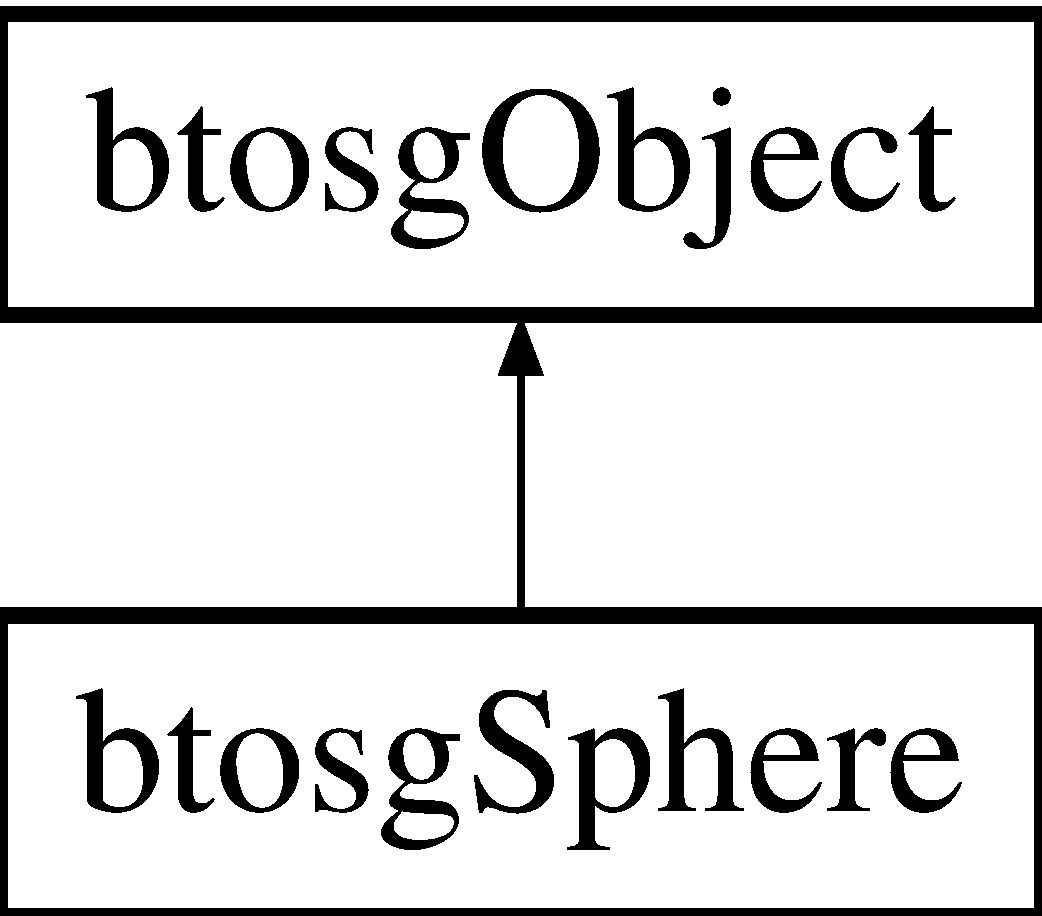
\includegraphics[height=2.000000cm]{classbtosgSphere}
\end{center}
\end{figure}
\subsection*{Public Member Functions}
\begin{DoxyCompactItemize}
\item 
\mbox{\Hypertarget{classbtosgSphere_a39cc5391405e85edcef16200b52e905c}\label{classbtosgSphere_a39cc5391405e85edcef16200b52e905c}} 
{\bfseries btosg\+Sphere} (float r)
\end{DoxyCompactItemize}
\subsection*{Public Attributes}
\begin{DoxyCompactItemize}
\item 
\mbox{\Hypertarget{classbtosgSphere_afd570c85e9ce1b15b2b4b378e4f6abeb}\label{classbtosgSphere_afd570c85e9ce1b15b2b4b378e4f6abeb}} 
float {\bfseries radius}
\end{DoxyCompactItemize}


The documentation for this class was generated from the following file\+:\begin{DoxyCompactItemize}
\item 
btosg.\+h\end{DoxyCompactItemize}

\hypertarget{classbtosgVehicle}{}\section{btosg\+Vehicle Class Reference}
\label{classbtosgVehicle}\index{btosg\+Vehicle@{btosg\+Vehicle}}


A four-\/wheeled vehicle based on bt\+Raycast\+Vehicle.  




{\ttfamily \#include $<$btosg\+Vehicle.\+h$>$}

Inheritance diagram for btosg\+Vehicle\+:\begin{figure}[H]
\begin{center}
\leavevmode
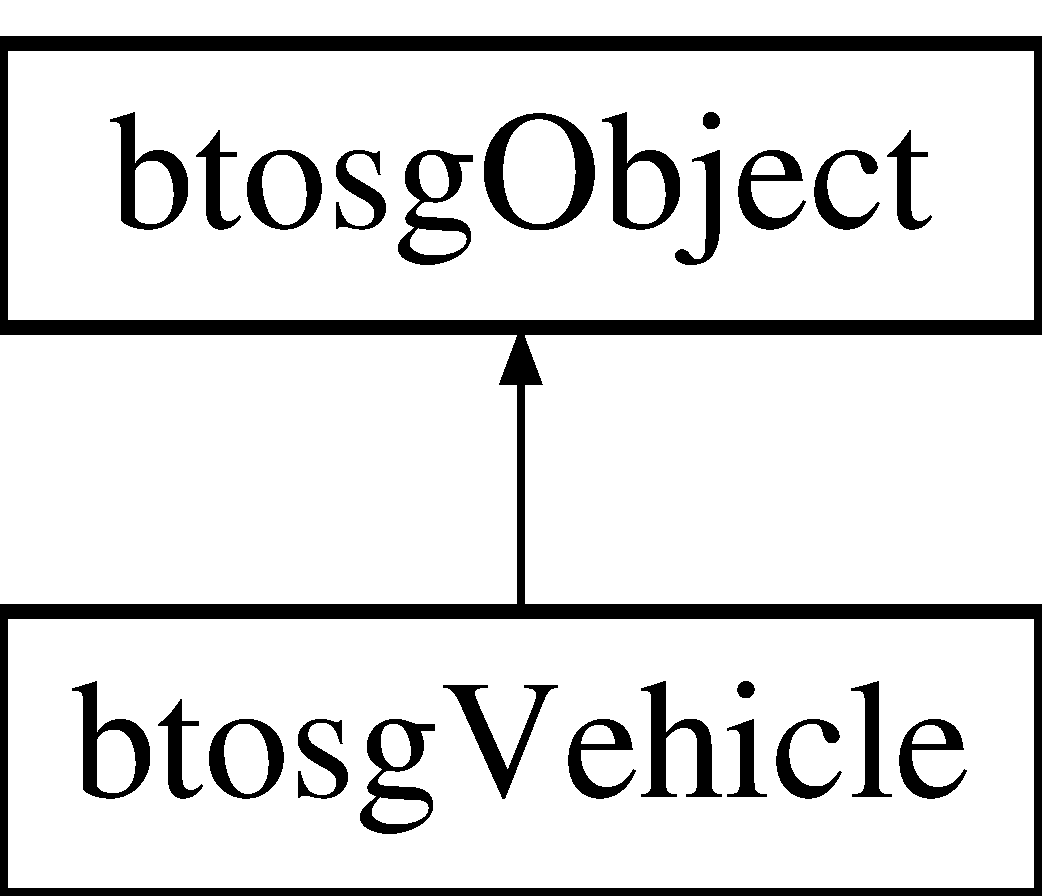
\includegraphics[height=2.000000cm]{classbtosgVehicle}
\end{center}
\end{figure}
\subsection*{Public Member Functions}
\begin{DoxyCompactItemize}
\item 
\hyperlink{classbtosgVehicle_aa754dd94553b8690763e4c24d1f26227}{btosg\+Vehicle} (\hyperlink{classbtosgWorld}{btosg\+World} $\ast$world, \hyperlink{classbtosgVec3}{btosg\+Vec3} dim\+Local=\hyperlink{classbtosgVec3}{btosg\+Vec3}(2., 0.\+4, 4.), double m=1000.)
\item 
void \hyperlink{classbtosgVehicle_a98971fb952c08cb72341a0c333fc66de}{add\+Wheels} (bt\+Vector3 $\ast$half\+Extents, bt\+Raycast\+Vehicle $\ast$\hyperlink{classbtosgVehicle_ac45b117f8b523f7040de99639deb7522}{vehicle}, bt\+Raycast\+Vehicle\+::bt\+Vehicle\+Tuning tuning)
\item 
void \hyperlink{classbtosgVehicle_abe98f64f0a8f37c7c0b244e3afbbcb15}{print\+Info} ()
\item 
void \hyperlink{classbtosgVehicle_ae9168c62263b26f95d068d94d6a7cab7}{log\+Position} ()
\item 
virtual void \hyperlink{classbtosgVehicle_a5fd0f471df492ac232c9b772a28bd2b9}{update} ()
\item 
void \hyperlink{classbtosgObject_ab06a1b3f357209214c6440cd5746523e}{set\+Name} (char const $\ast$n)
\item 
void \hyperlink{classbtosgObject_a91da93c82d48b86192f0cbb16054fe57}{set\+Mass} (double m)
\item 
\hyperlink{classbtosgVec3}{btosg\+Vec3} \hyperlink{classbtosgObject_a3dadd5da8f2a312e44a039446b93d4cd}{get\+Position} ()
\item 
\hyperlink{classbtosgQuat}{btosg\+Quat} \hyperlink{classbtosgObject_a3b825999ad3a51bde743d4085ff19dae}{get\+Rotation} ()
\item 
\hyperlink{classbtosgVec3}{btosg\+Vec3} \hyperlink{classbtosgObject_a2019ec63bde02b72600450c7c985e77a}{get\+Euler} ()
\item 
void \hyperlink{classbtosgObject_ace6b51040b7ddce90818174200cc6074}{set\+Position} (const \hyperlink{classbtosgVec3}{btosg\+Vec3} \&p)
\item 
void \hyperlink{classbtosgObject_adb9f2cff0faf66dc252cd7c97b11ac84}{set\+Position} (float x, float y, float z)
\item 
void \hyperlink{classbtosgObject_a6365748d5506bb9da31907c9988071fa}{set\+Rotation} (\hyperlink{classbtosgQuat}{btosg\+Quat} q)
\item 
void \hyperlink{classbtosgObject_a4d21ca59b944fd26644db35d3e9ba67a}{set\+Rotation} (float x, float y, float z, float w)
\item 
void \hyperlink{classbtosgObject_aff54acbc7c66811efb0cf2838107a241}{set\+Texture} (char const $\ast$fname)
\item 
void \hyperlink{classbtosgObject_a6ab7b9e0553dab398b980637788b56a8}{set\+Material} (osg\+::ref\+\_\+ptr$<$ osg\+::\+Material $>$ mat)
\item 
void \hyperlink{classbtosgObject_a93983f9180dd0672f8779cf2baa78580}{reset} ()
\item 
void \hyperlink{classbtosgObject_ad1508a0ce28cfac83e5f0ff6245f91b5}{set\+Init\+State} ()
\item 
void \hyperlink{classbtosgObject_a6ceb08e59ee95acaaef389ee198d2b56}{set\+Init\+State} (bt\+Transform i\+State)
\item 
void \hyperlink{classbtosgObject_a029dbe9134fa94e7355799f67fb2cd6d}{create\+Rigid\+Body} ()
\item 
void \hyperlink{classbtosgObject_a91838b8235579da178fcc06e6d3d47f3}{load\+Object\+Model} (char const $\ast$fname)
\end{DoxyCompactItemize}
\subsection*{Public Attributes}
\begin{DoxyCompactItemize}
\item 
float \hyperlink{classbtosgVehicle_aed23010bba3c34158abd4548328b3819}{dx}
\begin{DoxyCompactList}\small\item\em Vehicle x dimension. \end{DoxyCompactList}\item 
float \hyperlink{classbtosgVehicle_ae124e1cd8c424080d7be7c47edb07eb1}{dy}
\begin{DoxyCompactList}\small\item\em Vehicle y dimension. \end{DoxyCompactList}\item 
float \hyperlink{classbtosgVehicle_a39857392dc4882886964c1beefa46268}{dz}
\begin{DoxyCompactList}\small\item\em Vehicle $<$ dimension. \end{DoxyCompactList}\item 
\hyperlink{classbtosgVec3}{btosg\+Vec3} \hyperlink{classbtosgVehicle_a2173f99ca0719929aa5a1c890927aca3}{dim}
\begin{DoxyCompactList}\small\item\em Vehicle\textquotesingle{}s dimensions in world coordinates. \end{DoxyCompactList}\item 
\hyperlink{classbtosgVec3}{btosg\+Vec3} \hyperlink{classbtosgVehicle_a84705afaa9e37bb8a0bd7f6b6f291c26}{up}
\begin{DoxyCompactList}\small\item\em Vehicle\textquotesingle{}s up vector. Usually, up=-\/gravity. \end{DoxyCompactList}\item 
\hyperlink{classbtosgVec3}{btosg\+Vec3} \hyperlink{classbtosgVehicle_a33d6c0dc296ac54ec4a37e34332fa446}{front}
\begin{DoxyCompactList}\small\item\em Vehicle\textquotesingle{}s up vector. \end{DoxyCompactList}\item 
bt\+Raycast\+Vehicle $\ast$ \hyperlink{classbtosgVehicle_ac45b117f8b523f7040de99639deb7522}{vehicle}
\begin{DoxyCompactList}\small\item\em A bt\+Raycast\+Vehicle object. \end{DoxyCompactList}\item 
osg\+::ref\+\_\+ptr$<$ osg\+::\+Position\+Attitude\+Transform $>$ \hyperlink{classbtosgVehicle_a37edb4c28551037829ffd79c7bc315ba}{wheel} \mbox{[}4\mbox{]}
\begin{DoxyCompactList}\small\item\em Transformation from vehicle\textquotesingle{}s referential to wheel position. \end{DoxyCompactList}\item 
double \hyperlink{classbtosgVehicle_a0a9cd6f2c9b0defc44cd5e2e8d597418}{wheel\+Rotation} \mbox{[}4\mbox{]}
\begin{DoxyCompactList}\small\item\em Wheels\textquotesingle{} rotation angles. \end{DoxyCompactList}\item 
osg\+::ref\+\_\+ptr$<$ osg\+::\+Position\+Attitude\+Transform $>$ \hyperlink{classbtosgObject_afd15726e7a214212d6d5815f8ac1ac6c}{model}
\begin{DoxyCompactList}\small\item\em Object\textquotesingle{}s graphical model. \end{DoxyCompactList}\item 
char $\ast$ \hyperlink{classbtosgObject_a12396e1362797a75473a2e833b579cc9}{name}
\begin{DoxyCompactList}\small\item\em Object name. \end{DoxyCompactList}\item 
bt\+Transform \hyperlink{classbtosgObject_a2dee023f311114e200df9b04c8c1b400}{init\+\_\+state}
\begin{DoxyCompactList}\small\item\em Inital state. Applied on reset events. \end{DoxyCompactList}\item 
bt\+Rigid\+Body $\ast$ \hyperlink{classbtosgObject_a64ccde0543c184ed1749fdb9c9699785}{body}
\begin{DoxyCompactList}\small\item\em object\textquotesingle{}s rigid body \end{DoxyCompactList}\item 
bt\+Collision\+Shape $\ast$ \hyperlink{classbtosgObject_a0f6a8da01cf643c321bffe86e42604b0}{shape}
\begin{DoxyCompactList}\small\item\em Object\textquotesingle{}s collision shape. \end{DoxyCompactList}\item 
float \hyperlink{classbtosgObject_a2418bb2194d5e9b0f1c51c84672ba7d1}{mass}
\begin{DoxyCompactList}\small\item\em Mass of object. \end{DoxyCompactList}\end{DoxyCompactItemize}


\subsection{Detailed Description}
A four-\/wheeled vehicle based on bt\+Raycast\+Vehicle. 

\subsection{Constructor \& Destructor Documentation}
\mbox{\Hypertarget{classbtosgVehicle_aa754dd94553b8690763e4c24d1f26227}\label{classbtosgVehicle_aa754dd94553b8690763e4c24d1f26227}} 
\index{btosg\+Vehicle@{btosg\+Vehicle}!btosg\+Vehicle@{btosg\+Vehicle}}
\index{btosg\+Vehicle@{btosg\+Vehicle}!btosg\+Vehicle@{btosg\+Vehicle}}
\subsubsection{\texorpdfstring{btosg\+Vehicle()}{btosgVehicle()}}
{\footnotesize\ttfamily btosg\+Vehicle\+::btosg\+Vehicle (\begin{DoxyParamCaption}\item[{\hyperlink{classbtosgWorld}{btosg\+World} $\ast$}]{world,  }\item[{\hyperlink{classbtosgVec3}{btosg\+Vec3}}]{dim\+Local = {\ttfamily \hyperlink{classbtosgVec3}{btosg\+Vec3}(2.,0.4,4.)},  }\item[{double}]{m = {\ttfamily 1000.} }\end{DoxyParamCaption})\hspace{0.3cm}{\ttfamily [inline]}}

\hyperlink{classbtosgVehicle}{btosg\+Vehicle} constructor. 

References add\+Wheels(), btosg\+Object\+::body, btosg\+Object\+::create\+Rigid\+Body(), btosg\+World\+::dynamic, btosg\+Object\+::model, btosg\+Object\+::set\+Mass(), btosg\+Object\+::set\+Material(), and btosg\+Object\+::shape.



\subsection{Member Function Documentation}
\mbox{\Hypertarget{classbtosgVehicle_a98971fb952c08cb72341a0c333fc66de}\label{classbtosgVehicle_a98971fb952c08cb72341a0c333fc66de}} 
\index{btosg\+Vehicle@{btosg\+Vehicle}!add\+Wheels@{add\+Wheels}}
\index{add\+Wheels@{add\+Wheels}!btosg\+Vehicle@{btosg\+Vehicle}}
\subsubsection{\texorpdfstring{add\+Wheels()}{addWheels()}}
{\footnotesize\ttfamily void btosg\+Vehicle\+::add\+Wheels (\begin{DoxyParamCaption}\item[{bt\+Vector3 $\ast$}]{half\+Extents,  }\item[{bt\+Raycast\+Vehicle $\ast$}]{vehicle,  }\item[{bt\+Raycast\+Vehicle\+::bt\+Vehicle\+Tuning}]{tuning }\end{DoxyParamCaption})\hspace{0.3cm}{\ttfamily [inline]}}

Adds four wheels to the vehicle. 

References btosg\+Object\+::model.



Referenced by btosg\+Vehicle().

\mbox{\Hypertarget{classbtosgObject_a029dbe9134fa94e7355799f67fb2cd6d}\label{classbtosgObject_a029dbe9134fa94e7355799f67fb2cd6d}} 
\index{btosg\+Vehicle@{btosg\+Vehicle}!create\+Rigid\+Body@{create\+Rigid\+Body}}
\index{create\+Rigid\+Body@{create\+Rigid\+Body}!btosg\+Vehicle@{btosg\+Vehicle}}
\subsubsection{\texorpdfstring{create\+Rigid\+Body()}{createRigidBody()}}
{\footnotesize\ttfamily void btosg\+Object\+::create\+Rigid\+Body (\begin{DoxyParamCaption}{ }\end{DoxyParamCaption})\hspace{0.3cm}{\ttfamily [inline]}, {\ttfamily [inherited]}}

Creates a new rigid body as a bt\+Rigid\+Body object. 

Referenced by btosg\+Vehicle().

\mbox{\Hypertarget{classbtosgObject_a2019ec63bde02b72600450c7c985e77a}\label{classbtosgObject_a2019ec63bde02b72600450c7c985e77a}} 
\index{btosg\+Vehicle@{btosg\+Vehicle}!get\+Euler@{get\+Euler}}
\index{get\+Euler@{get\+Euler}!btosg\+Vehicle@{btosg\+Vehicle}}
\subsubsection{\texorpdfstring{get\+Euler()}{getEuler()}}
{\footnotesize\ttfamily \hyperlink{classbtosgVec3}{btosg\+Vec3} btosg\+Object\+::get\+Euler (\begin{DoxyParamCaption}{ }\end{DoxyParamCaption})\hspace{0.3cm}{\ttfamily [inline]}, {\ttfamily [inherited]}}

Returns object\textquotesingle{}s attitude as H\+PR Euler angles. 

References btosg\+Quat\+::to\+Euler().

\mbox{\Hypertarget{classbtosgObject_a3dadd5da8f2a312e44a039446b93d4cd}\label{classbtosgObject_a3dadd5da8f2a312e44a039446b93d4cd}} 
\index{btosg\+Vehicle@{btosg\+Vehicle}!get\+Position@{get\+Position}}
\index{get\+Position@{get\+Position}!btosg\+Vehicle@{btosg\+Vehicle}}
\subsubsection{\texorpdfstring{get\+Position()}{getPosition()}}
{\footnotesize\ttfamily \hyperlink{classbtosgVec3}{btosg\+Vec3} btosg\+Object\+::get\+Position (\begin{DoxyParamCaption}{ }\end{DoxyParamCaption})\hspace{0.3cm}{\ttfamily [inline]}, {\ttfamily [inherited]}}

Returns object\textquotesingle{}s position. 

References btosg\+Vec3\+::btosg\+Vec3().

\mbox{\Hypertarget{classbtosgObject_a3b825999ad3a51bde743d4085ff19dae}\label{classbtosgObject_a3b825999ad3a51bde743d4085ff19dae}} 
\index{btosg\+Vehicle@{btosg\+Vehicle}!get\+Rotation@{get\+Rotation}}
\index{get\+Rotation@{get\+Rotation}!btosg\+Vehicle@{btosg\+Vehicle}}
\subsubsection{\texorpdfstring{get\+Rotation()}{getRotation()}}
{\footnotesize\ttfamily \hyperlink{classbtosgQuat}{btosg\+Quat} btosg\+Object\+::get\+Rotation (\begin{DoxyParamCaption}{ }\end{DoxyParamCaption})\hspace{0.3cm}{\ttfamily [inline]}, {\ttfamily [inherited]}}

Returns object\textquotesingle{}s attitude as a Quaternion. \mbox{\Hypertarget{classbtosgObject_a91838b8235579da178fcc06e6d3d47f3}\label{classbtosgObject_a91838b8235579da178fcc06e6d3d47f3}} 
\index{btosg\+Vehicle@{btosg\+Vehicle}!load\+Object\+Model@{load\+Object\+Model}}
\index{load\+Object\+Model@{load\+Object\+Model}!btosg\+Vehicle@{btosg\+Vehicle}}
\subsubsection{\texorpdfstring{load\+Object\+Model()}{loadObjectModel()}}
{\footnotesize\ttfamily void btosg\+Object\+::load\+Object\+Model (\begin{DoxyParamCaption}\item[{char const $\ast$}]{fname }\end{DoxyParamCaption})\hspace{0.3cm}{\ttfamily [inherited]}}

Loads an object model from a Wavefront O\+BJ file. Loadded model is used to define both the collision and graphical shapes. \mbox{\Hypertarget{classbtosgVehicle_ae9168c62263b26f95d068d94d6a7cab7}\label{classbtosgVehicle_ae9168c62263b26f95d068d94d6a7cab7}} 
\index{btosg\+Vehicle@{btosg\+Vehicle}!log\+Position@{log\+Position}}
\index{log\+Position@{log\+Position}!btosg\+Vehicle@{btosg\+Vehicle}}
\subsubsection{\texorpdfstring{log\+Position()}{logPosition()}}
{\footnotesize\ttfamily void btosg\+Vehicle\+::log\+Position (\begin{DoxyParamCaption}{ }\end{DoxyParamCaption})\hspace{0.3cm}{\ttfamily [inline]}}

Outputs vehicle\textquotesingle{}s position. 

References btosg\+Object\+::body, and btosg\+Object\+::name.

\mbox{\Hypertarget{classbtosgVehicle_abe98f64f0a8f37c7c0b244e3afbbcb15}\label{classbtosgVehicle_abe98f64f0a8f37c7c0b244e3afbbcb15}} 
\index{btosg\+Vehicle@{btosg\+Vehicle}!print\+Info@{print\+Info}}
\index{print\+Info@{print\+Info}!btosg\+Vehicle@{btosg\+Vehicle}}
\subsubsection{\texorpdfstring{print\+Info()}{printInfo()}}
{\footnotesize\ttfamily void btosg\+Vehicle\+::print\+Info (\begin{DoxyParamCaption}{ }\end{DoxyParamCaption})\hspace{0.3cm}{\ttfamily [inline]}}

Outputs vehicle\textquotesingle{}s info. 

References btosg\+Object\+::body, and btosg\+Object\+::mass.

\mbox{\Hypertarget{classbtosgObject_a93983f9180dd0672f8779cf2baa78580}\label{classbtosgObject_a93983f9180dd0672f8779cf2baa78580}} 
\index{btosg\+Vehicle@{btosg\+Vehicle}!reset@{reset}}
\index{reset@{reset}!btosg\+Vehicle@{btosg\+Vehicle}}
\subsubsection{\texorpdfstring{reset()}{reset()}}
{\footnotesize\ttfamily void btosg\+Object\+::reset (\begin{DoxyParamCaption}{ }\end{DoxyParamCaption})\hspace{0.3cm}{\ttfamily [inline]}, {\ttfamily [inherited]}}

Reposition object to its inital state. 

References btosg\+Vec3\+::btosg\+Vec3().



Referenced by btosg\+World\+::reset().

\mbox{\Hypertarget{classbtosgObject_ad1508a0ce28cfac83e5f0ff6245f91b5}\label{classbtosgObject_ad1508a0ce28cfac83e5f0ff6245f91b5}} 
\index{btosg\+Vehicle@{btosg\+Vehicle}!set\+Init\+State@{set\+Init\+State}}
\index{set\+Init\+State@{set\+Init\+State}!btosg\+Vehicle@{btosg\+Vehicle}}
\subsubsection{\texorpdfstring{set\+Init\+State()}{setInitState()}\hspace{0.1cm}{\footnotesize\ttfamily [1/2]}}
{\footnotesize\ttfamily void btosg\+Object\+::set\+Init\+State (\begin{DoxyParamCaption}{ }\end{DoxyParamCaption})\hspace{0.3cm}{\ttfamily [inline]}, {\ttfamily [inherited]}}

Stores current state as init state. Init state is aplied by \hyperlink{classbtosgObject_a93983f9180dd0672f8779cf2baa78580}{reset()} 

Referenced by btosg\+World\+::step\+Simulation().

\mbox{\Hypertarget{classbtosgObject_a6ceb08e59ee95acaaef389ee198d2b56}\label{classbtosgObject_a6ceb08e59ee95acaaef389ee198d2b56}} 
\index{btosg\+Vehicle@{btosg\+Vehicle}!set\+Init\+State@{set\+Init\+State}}
\index{set\+Init\+State@{set\+Init\+State}!btosg\+Vehicle@{btosg\+Vehicle}}
\subsubsection{\texorpdfstring{set\+Init\+State()}{setInitState()}\hspace{0.1cm}{\footnotesize\ttfamily [2/2]}}
{\footnotesize\ttfamily void btosg\+Object\+::set\+Init\+State (\begin{DoxyParamCaption}\item[{bt\+Transform}]{i\+State }\end{DoxyParamCaption})\hspace{0.3cm}{\ttfamily [inline]}, {\ttfamily [inherited]}}

Stores i\+State as init state. Init state is aplied by \hyperlink{classbtosgObject_a93983f9180dd0672f8779cf2baa78580}{reset()} \mbox{\Hypertarget{classbtosgObject_a91da93c82d48b86192f0cbb16054fe57}\label{classbtosgObject_a91da93c82d48b86192f0cbb16054fe57}} 
\index{btosg\+Vehicle@{btosg\+Vehicle}!set\+Mass@{set\+Mass}}
\index{set\+Mass@{set\+Mass}!btosg\+Vehicle@{btosg\+Vehicle}}
\subsubsection{\texorpdfstring{set\+Mass()}{setMass()}}
{\footnotesize\ttfamily void btosg\+Object\+::set\+Mass (\begin{DoxyParamCaption}\item[{double}]{m }\end{DoxyParamCaption})\hspace{0.3cm}{\ttfamily [inline]}, {\ttfamily [inherited]}}

Sets the object\textquotesingle{}s mass. 

Referenced by btosg\+Vehicle().

\mbox{\Hypertarget{classbtosgObject_a6ab7b9e0553dab398b980637788b56a8}\label{classbtosgObject_a6ab7b9e0553dab398b980637788b56a8}} 
\index{btosg\+Vehicle@{btosg\+Vehicle}!set\+Material@{set\+Material}}
\index{set\+Material@{set\+Material}!btosg\+Vehicle@{btosg\+Vehicle}}
\subsubsection{\texorpdfstring{set\+Material()}{setMaterial()}}
{\footnotesize\ttfamily void btosg\+Object\+::set\+Material (\begin{DoxyParamCaption}\item[{osg\+::ref\+\_\+ptr$<$ osg\+::\+Material $>$}]{mat }\end{DoxyParamCaption})\hspace{0.3cm}{\ttfamily [inline]}, {\ttfamily [inherited]}}

Sets the material properties for the object. 

Referenced by btosg\+Vehicle().

\mbox{\Hypertarget{classbtosgObject_ab06a1b3f357209214c6440cd5746523e}\label{classbtosgObject_ab06a1b3f357209214c6440cd5746523e}} 
\index{btosg\+Vehicle@{btosg\+Vehicle}!set\+Name@{set\+Name}}
\index{set\+Name@{set\+Name}!btosg\+Vehicle@{btosg\+Vehicle}}
\subsubsection{\texorpdfstring{set\+Name()}{setName()}}
{\footnotesize\ttfamily void btosg\+Object\+::set\+Name (\begin{DoxyParamCaption}\item[{char const $\ast$}]{n }\end{DoxyParamCaption})\hspace{0.3cm}{\ttfamily [inline]}, {\ttfamily [inherited]}}

Sets the object\textquotesingle{}s name. \mbox{\Hypertarget{classbtosgObject_ace6b51040b7ddce90818174200cc6074}\label{classbtosgObject_ace6b51040b7ddce90818174200cc6074}} 
\index{btosg\+Vehicle@{btosg\+Vehicle}!set\+Position@{set\+Position}}
\index{set\+Position@{set\+Position}!btosg\+Vehicle@{btosg\+Vehicle}}
\subsubsection{\texorpdfstring{set\+Position()}{setPosition()}\hspace{0.1cm}{\footnotesize\ttfamily [1/2]}}
{\footnotesize\ttfamily void btosg\+Object\+::set\+Position (\begin{DoxyParamCaption}\item[{const \hyperlink{classbtosgVec3}{btosg\+Vec3} \&}]{p }\end{DoxyParamCaption})\hspace{0.3cm}{\ttfamily [inline]}, {\ttfamily [inherited]}}

Sets objects position. \mbox{\Hypertarget{classbtosgObject_adb9f2cff0faf66dc252cd7c97b11ac84}\label{classbtosgObject_adb9f2cff0faf66dc252cd7c97b11ac84}} 
\index{btosg\+Vehicle@{btosg\+Vehicle}!set\+Position@{set\+Position}}
\index{set\+Position@{set\+Position}!btosg\+Vehicle@{btosg\+Vehicle}}
\subsubsection{\texorpdfstring{set\+Position()}{setPosition()}\hspace{0.1cm}{\footnotesize\ttfamily [2/2]}}
{\footnotesize\ttfamily void btosg\+Object\+::set\+Position (\begin{DoxyParamCaption}\item[{float}]{x,  }\item[{float}]{y,  }\item[{float}]{z }\end{DoxyParamCaption})\hspace{0.3cm}{\ttfamily [inline]}, {\ttfamily [inherited]}}

Sets objects position. 

References btosg\+Vec3\+::btosg\+Vec3().

\mbox{\Hypertarget{classbtosgObject_a6365748d5506bb9da31907c9988071fa}\label{classbtosgObject_a6365748d5506bb9da31907c9988071fa}} 
\index{btosg\+Vehicle@{btosg\+Vehicle}!set\+Rotation@{set\+Rotation}}
\index{set\+Rotation@{set\+Rotation}!btosg\+Vehicle@{btosg\+Vehicle}}
\subsubsection{\texorpdfstring{set\+Rotation()}{setRotation()}\hspace{0.1cm}{\footnotesize\ttfamily [1/2]}}
{\footnotesize\ttfamily void btosg\+Object\+::set\+Rotation (\begin{DoxyParamCaption}\item[{\hyperlink{classbtosgQuat}{btosg\+Quat}}]{q }\end{DoxyParamCaption})\hspace{0.3cm}{\ttfamily [inline]}, {\ttfamily [inherited]}}

Sets objects attitude from a quaternion. \mbox{\Hypertarget{classbtosgObject_a4d21ca59b944fd26644db35d3e9ba67a}\label{classbtosgObject_a4d21ca59b944fd26644db35d3e9ba67a}} 
\index{btosg\+Vehicle@{btosg\+Vehicle}!set\+Rotation@{set\+Rotation}}
\index{set\+Rotation@{set\+Rotation}!btosg\+Vehicle@{btosg\+Vehicle}}
\subsubsection{\texorpdfstring{set\+Rotation()}{setRotation()}\hspace{0.1cm}{\footnotesize\ttfamily [2/2]}}
{\footnotesize\ttfamily void btosg\+Object\+::set\+Rotation (\begin{DoxyParamCaption}\item[{float}]{x,  }\item[{float}]{y,  }\item[{float}]{z,  }\item[{float}]{w }\end{DoxyParamCaption})\hspace{0.3cm}{\ttfamily [inline]}, {\ttfamily [inherited]}}

Sets objects attitude from the quaternion coords. \mbox{\Hypertarget{classbtosgObject_aff54acbc7c66811efb0cf2838107a241}\label{classbtosgObject_aff54acbc7c66811efb0cf2838107a241}} 
\index{btosg\+Vehicle@{btosg\+Vehicle}!set\+Texture@{set\+Texture}}
\index{set\+Texture@{set\+Texture}!btosg\+Vehicle@{btosg\+Vehicle}}
\subsubsection{\texorpdfstring{set\+Texture()}{setTexture()}}
{\footnotesize\ttfamily void btosg\+Object\+::set\+Texture (\begin{DoxyParamCaption}\item[{char const $\ast$}]{fname }\end{DoxyParamCaption})\hspace{0.3cm}{\ttfamily [inherited]}}

Sets the object texture from a loaded image file. \mbox{\Hypertarget{classbtosgVehicle_a5fd0f471df492ac232c9b772a28bd2b9}\label{classbtosgVehicle_a5fd0f471df492ac232c9b772a28bd2b9}} 
\index{btosg\+Vehicle@{btosg\+Vehicle}!update@{update}}
\index{update@{update}!btosg\+Vehicle@{btosg\+Vehicle}}
\subsubsection{\texorpdfstring{update()}{update()}}
{\footnotesize\ttfamily virtual void btosg\+Vehicle\+::update (\begin{DoxyParamCaption}{ }\end{DoxyParamCaption})\hspace{0.3cm}{\ttfamily [inline]}, {\ttfamily [virtual]}}

Vehicle\textquotesingle{}s update callback. This function is called automatically from World\+::setp\+Simulation() for each registered vehicle. Positions graphical vehicle and wheels from their physhical states. 

Reimplemented from \hyperlink{classbtosgObject_a342917817dfde62554f83da8e0d5110b}{btosg\+Object}.



References btosg\+Object\+::update().



\subsection{Member Data Documentation}
\mbox{\Hypertarget{classbtosgObject_a64ccde0543c184ed1749fdb9c9699785}\label{classbtosgObject_a64ccde0543c184ed1749fdb9c9699785}} 
\index{btosg\+Vehicle@{btosg\+Vehicle}!body@{body}}
\index{body@{body}!btosg\+Vehicle@{btosg\+Vehicle}}
\subsubsection{\texorpdfstring{body}{body}}
{\footnotesize\ttfamily bt\+Rigid\+Body$\ast$ btosg\+Object\+::body\hspace{0.3cm}{\ttfamily [inherited]}}



object\textquotesingle{}s rigid body 



Referenced by btosg\+World\+::add\+Object(), btosg\+Vehicle(), log\+Position(), and print\+Info().

\mbox{\Hypertarget{classbtosgVehicle_a2173f99ca0719929aa5a1c890927aca3}\label{classbtosgVehicle_a2173f99ca0719929aa5a1c890927aca3}} 
\index{btosg\+Vehicle@{btosg\+Vehicle}!dim@{dim}}
\index{dim@{dim}!btosg\+Vehicle@{btosg\+Vehicle}}
\subsubsection{\texorpdfstring{dim}{dim}}
{\footnotesize\ttfamily \hyperlink{classbtosgVec3}{btosg\+Vec3} btosg\+Vehicle\+::dim}



Vehicle\textquotesingle{}s dimensions in world coordinates. 

\mbox{\Hypertarget{classbtosgVehicle_aed23010bba3c34158abd4548328b3819}\label{classbtosgVehicle_aed23010bba3c34158abd4548328b3819}} 
\index{btosg\+Vehicle@{btosg\+Vehicle}!dx@{dx}}
\index{dx@{dx}!btosg\+Vehicle@{btosg\+Vehicle}}
\subsubsection{\texorpdfstring{dx}{dx}}
{\footnotesize\ttfamily float btosg\+Vehicle\+::dx}



Vehicle x dimension. 

\mbox{\Hypertarget{classbtosgVehicle_ae124e1cd8c424080d7be7c47edb07eb1}\label{classbtosgVehicle_ae124e1cd8c424080d7be7c47edb07eb1}} 
\index{btosg\+Vehicle@{btosg\+Vehicle}!dy@{dy}}
\index{dy@{dy}!btosg\+Vehicle@{btosg\+Vehicle}}
\subsubsection{\texorpdfstring{dy}{dy}}
{\footnotesize\ttfamily float btosg\+Vehicle\+::dy}



Vehicle y dimension. 

\mbox{\Hypertarget{classbtosgVehicle_a39857392dc4882886964c1beefa46268}\label{classbtosgVehicle_a39857392dc4882886964c1beefa46268}} 
\index{btosg\+Vehicle@{btosg\+Vehicle}!dz@{dz}}
\index{dz@{dz}!btosg\+Vehicle@{btosg\+Vehicle}}
\subsubsection{\texorpdfstring{dz}{dz}}
{\footnotesize\ttfamily float btosg\+Vehicle\+::dz}



Vehicle $<$ dimension. 

\mbox{\Hypertarget{classbtosgVehicle_a33d6c0dc296ac54ec4a37e34332fa446}\label{classbtosgVehicle_a33d6c0dc296ac54ec4a37e34332fa446}} 
\index{btosg\+Vehicle@{btosg\+Vehicle}!front@{front}}
\index{front@{front}!btosg\+Vehicle@{btosg\+Vehicle}}
\subsubsection{\texorpdfstring{front}{front}}
{\footnotesize\ttfamily \hyperlink{classbtosgVec3}{btosg\+Vec3} btosg\+Vehicle\+::front}



Vehicle\textquotesingle{}s up vector. 

\mbox{\Hypertarget{classbtosgObject_a2dee023f311114e200df9b04c8c1b400}\label{classbtosgObject_a2dee023f311114e200df9b04c8c1b400}} 
\index{btosg\+Vehicle@{btosg\+Vehicle}!init\+\_\+state@{init\+\_\+state}}
\index{init\+\_\+state@{init\+\_\+state}!btosg\+Vehicle@{btosg\+Vehicle}}
\subsubsection{\texorpdfstring{init\+\_\+state}{init\_state}}
{\footnotesize\ttfamily bt\+Transform btosg\+Object\+::init\+\_\+state\hspace{0.3cm}{\ttfamily [inherited]}}



Inital state. Applied on reset events. 

\mbox{\Hypertarget{classbtosgObject_a2418bb2194d5e9b0f1c51c84672ba7d1}\label{classbtosgObject_a2418bb2194d5e9b0f1c51c84672ba7d1}} 
\index{btosg\+Vehicle@{btosg\+Vehicle}!mass@{mass}}
\index{mass@{mass}!btosg\+Vehicle@{btosg\+Vehicle}}
\subsubsection{\texorpdfstring{mass}{mass}}
{\footnotesize\ttfamily float btosg\+Object\+::mass\hspace{0.3cm}{\ttfamily [inherited]}}



Mass of object. 



Referenced by print\+Info().

\mbox{\Hypertarget{classbtosgObject_afd15726e7a214212d6d5815f8ac1ac6c}\label{classbtosgObject_afd15726e7a214212d6d5815f8ac1ac6c}} 
\index{btosg\+Vehicle@{btosg\+Vehicle}!model@{model}}
\index{model@{model}!btosg\+Vehicle@{btosg\+Vehicle}}
\subsubsection{\texorpdfstring{model}{model}}
{\footnotesize\ttfamily osg\+::ref\+\_\+ptr$<$osg\+::\+Position\+Attitude\+Transform$>$ btosg\+Object\+::model\hspace{0.3cm}{\ttfamily [inherited]}}



Object\textquotesingle{}s graphical model. 



Referenced by btosg\+World\+::add\+Object(), add\+Wheels(), and btosg\+Vehicle().

\mbox{\Hypertarget{classbtosgObject_a12396e1362797a75473a2e833b579cc9}\label{classbtosgObject_a12396e1362797a75473a2e833b579cc9}} 
\index{btosg\+Vehicle@{btosg\+Vehicle}!name@{name}}
\index{name@{name}!btosg\+Vehicle@{btosg\+Vehicle}}
\subsubsection{\texorpdfstring{name}{name}}
{\footnotesize\ttfamily char$\ast$ btosg\+Object\+::name\hspace{0.3cm}{\ttfamily [inherited]}}



Object name. 



Referenced by log\+Position().

\mbox{\Hypertarget{classbtosgObject_a0f6a8da01cf643c321bffe86e42604b0}\label{classbtosgObject_a0f6a8da01cf643c321bffe86e42604b0}} 
\index{btosg\+Vehicle@{btosg\+Vehicle}!shape@{shape}}
\index{shape@{shape}!btosg\+Vehicle@{btosg\+Vehicle}}
\subsubsection{\texorpdfstring{shape}{shape}}
{\footnotesize\ttfamily bt\+Collision\+Shape$\ast$ btosg\+Object\+::shape\hspace{0.3cm}{\ttfamily [inherited]}}



Object\textquotesingle{}s collision shape. 



Referenced by btosg\+Vehicle().

\mbox{\Hypertarget{classbtosgVehicle_a84705afaa9e37bb8a0bd7f6b6f291c26}\label{classbtosgVehicle_a84705afaa9e37bb8a0bd7f6b6f291c26}} 
\index{btosg\+Vehicle@{btosg\+Vehicle}!up@{up}}
\index{up@{up}!btosg\+Vehicle@{btosg\+Vehicle}}
\subsubsection{\texorpdfstring{up}{up}}
{\footnotesize\ttfamily \hyperlink{classbtosgVec3}{btosg\+Vec3} btosg\+Vehicle\+::up}



Vehicle\textquotesingle{}s up vector. Usually, up=-\/gravity. 

\mbox{\Hypertarget{classbtosgVehicle_ac45b117f8b523f7040de99639deb7522}\label{classbtosgVehicle_ac45b117f8b523f7040de99639deb7522}} 
\index{btosg\+Vehicle@{btosg\+Vehicle}!vehicle@{vehicle}}
\index{vehicle@{vehicle}!btosg\+Vehicle@{btosg\+Vehicle}}
\subsubsection{\texorpdfstring{vehicle}{vehicle}}
{\footnotesize\ttfamily bt\+Raycast\+Vehicle$\ast$ btosg\+Vehicle\+::vehicle}



A bt\+Raycast\+Vehicle object. 

\mbox{\Hypertarget{classbtosgVehicle_a37edb4c28551037829ffd79c7bc315ba}\label{classbtosgVehicle_a37edb4c28551037829ffd79c7bc315ba}} 
\index{btosg\+Vehicle@{btosg\+Vehicle}!wheel@{wheel}}
\index{wheel@{wheel}!btosg\+Vehicle@{btosg\+Vehicle}}
\subsubsection{\texorpdfstring{wheel}{wheel}}
{\footnotesize\ttfamily osg\+::ref\+\_\+ptr$<$osg\+::\+Position\+Attitude\+Transform$>$ btosg\+Vehicle\+::wheel\mbox{[}4\mbox{]}}



Transformation from vehicle\textquotesingle{}s referential to wheel position. 

\mbox{\Hypertarget{classbtosgVehicle_a0a9cd6f2c9b0defc44cd5e2e8d597418}\label{classbtosgVehicle_a0a9cd6f2c9b0defc44cd5e2e8d597418}} 
\index{btosg\+Vehicle@{btosg\+Vehicle}!wheel\+Rotation@{wheel\+Rotation}}
\index{wheel\+Rotation@{wheel\+Rotation}!btosg\+Vehicle@{btosg\+Vehicle}}
\subsubsection{\texorpdfstring{wheel\+Rotation}{wheelRotation}}
{\footnotesize\ttfamily double btosg\+Vehicle\+::wheel\+Rotation\mbox{[}4\mbox{]}}



Wheels\textquotesingle{} rotation angles. 



The documentation for this class was generated from the following file\+:\begin{DoxyCompactItemize}
\item 
btosg\+Vehicle.\+h (/$\ast$
	btosg\+Vehicle.\+h
	\+Miguel Leitao, 2016
$\ast$/

\#ifndef B\+T\+O\+S\+G\+V\+E\+H\+I\+C\+L\+E\+\_\+\+H
\#define B\+T\+O\+S\+G\+V\+E\+H\+I\+C\+L\+E\+\_\+\+H 1

\#include $<$osg/\+Material$>$

\#include $<$bt\+Bullet\+Collision\+Common.\+h$>$
\#include $<$bt\+Bullet\+Dynamics\+Common.\+h$>$
\#include $<$\+Bullet\+Dynamics/\+Vehicle/bt\+Rayca

\#include \char`\"{}btosg.\+h\char`\"{}

\#include $<$osg/\+Material$>$
\#include $<$osg/\+Texture2\+D$>$

/$\ast$
class btosg\+Wheel \+: public btosg\+Cylinder 
    public\+:
        btosg\+Wheel(bt\+Vector3 pos, double
            set\+Position(pos);
            set\+Rotation(osg\+::\+Quat(ang,os
            set\+Texture(\char`\"{}wheel.\+png\char`\"{});
            body-\/$>$set\+Friction(100.);
        \}
        virtual void update() \{
        if (body) \{
            bt\+Transform w\+Trans;
            body-\/$>$get\+Motion\+State()-\/$>$get\+W

            if ( model ) \{
                model-\/$>$set\+Attitude(bt2os
                model-\/$>$set\+Position(bt2os
            \}
            //log\+Position();

        \}
    \}
\};
$\ast$/

/// A four-\/wheeled vehicle based on bt\+Ra
class btosg\+Vehicle\+: public btosg\+Object \{
private\+:
    bt\+Default\+Vehicle\+Raycaster $\ast$ray\+Caster
public\+:
    float dx;			///$<$ Vehic)\end{DoxyCompactItemize}

\hypertarget{classbtosgWorld}{}\section{btosg\+World Class Reference}
\label{classbtosgWorld}\index{btosg\+World@{btosg\+World}}
\subsection*{Public Member Functions}
\begin{DoxyCompactItemize}
\item 
void \hyperlink{classbtosgWorld_afce096686d8f84afd8b8fa3f2dc161b8}{step\+Simulation} (bt\+Scalar time\+Step, int max\+Sub\+Steps)
\item 
void \hyperlink{classbtosgWorld_ae5b71c6319dd420479096a265a1725b7}{add\+Object} (class \hyperlink{classbtosgObject}{btosg\+Object} $\ast$obj)
\item 
void \hyperlink{classbtosgWorld_a6af4d066410a86b44fff5563667ea9a9}{reset} ()
\end{DoxyCompactItemize}
\subsection*{Public Attributes}
\begin{DoxyCompactItemize}
\item 
\mbox{\Hypertarget{classbtosgWorld_ad757a7b3b845142f200d1f2127e5372e}\label{classbtosgWorld_ad757a7b3b845142f200d1f2127e5372e}} 
bt\+Dynamics\+World $\ast$ {\bfseries dynamic}
\item 
\mbox{\Hypertarget{classbtosgWorld_ab6d438f54ccfc18955ea43e87731e008}\label{classbtosgWorld_ab6d438f54ccfc18955ea43e87731e008}} 
osg\+::ref\+\_\+ptr$<$ osg\+::\+Group $>$ {\bfseries scene}
\item 
\mbox{\Hypertarget{classbtosgWorld_ab105aa8c0f8bdbdf323d47b902f6aca0}\label{classbtosgWorld_ab105aa8c0f8bdbdf323d47b902f6aca0}} 
std\+::forward\+\_\+list$<$ class \hyperlink{classbtosgObject}{btosg\+Object} $\ast$ $>$ {\bfseries objects}
\end{DoxyCompactItemize}


\subsection{Member Function Documentation}
\mbox{\Hypertarget{classbtosgWorld_ae5b71c6319dd420479096a265a1725b7}\label{classbtosgWorld_ae5b71c6319dd420479096a265a1725b7}} 
\index{btosg\+World@{btosg\+World}!add\+Object@{add\+Object}}
\index{add\+Object@{add\+Object}!btosg\+World@{btosg\+World}}
\subsubsection{\texorpdfstring{add\+Object()}{addObject()}}
{\footnotesize\ttfamily void btosg\+World\+::add\+Object (\begin{DoxyParamCaption}\item[{class \hyperlink{classbtosgObject}{btosg\+Object} $\ast$}]{obj }\end{DoxyParamCaption})}

Registers the object obj into a simulation world. \mbox{\Hypertarget{classbtosgWorld_a6af4d066410a86b44fff5563667ea9a9}\label{classbtosgWorld_a6af4d066410a86b44fff5563667ea9a9}} 
\index{btosg\+World@{btosg\+World}!reset@{reset}}
\index{reset@{reset}!btosg\+World@{btosg\+World}}
\subsubsection{\texorpdfstring{reset()}{reset()}}
{\footnotesize\ttfamily void btosg\+World\+::reset (\begin{DoxyParamCaption}{ }\end{DoxyParamCaption})}

Reset all registered objects. \mbox{\Hypertarget{classbtosgWorld_afce096686d8f84afd8b8fa3f2dc161b8}\label{classbtosgWorld_afce096686d8f84afd8b8fa3f2dc161b8}} 
\index{btosg\+World@{btosg\+World}!step\+Simulation@{step\+Simulation}}
\index{step\+Simulation@{step\+Simulation}!btosg\+World@{btosg\+World}}
\subsubsection{\texorpdfstring{step\+Simulation()}{stepSimulation()}}
{\footnotesize\ttfamily void btosg\+World\+::step\+Simulation (\begin{DoxyParamCaption}\item[{bt\+Scalar}]{time\+Step,  }\item[{int}]{max\+Sub\+Steps }\end{DoxyParamCaption})}

Performs a simulation step. 

The documentation for this class was generated from the following files\+:\begin{DoxyCompactItemize}
\item 
btosg.\+h\item 
btosg.\+cpp\end{DoxyCompactItemize}

%--- End generated contents ---

% Index
\backmatter
\newpage
\phantomsection
\clearemptydoublepage
\addcontentsline{toc}{chapter}{Index}
\printindex

\end{document}
